% !TeX root = RJwrapper.tex
\title{\pkg{ClusTorus}: An R Package for Prediction and Clustering on the Torus by Conformal Prediction}
\author{by Seungki Hong and Sungkyu Jung}

\maketitle

\abstract{Protein structure data consist of several dihedral angles, lying on a multidimensional torus. Analyzing such data has been and continues to be key in understanding functional properties of proteins. However, most of the existing statistical methods assume that data are on Euclidean spaces, and thus they are improper to deal with angular data. In this paper, we introduce the package \pkg{ClusTorus} specialized to analyzing multivariate angular data. The package collects some tools and routines to perform algorithmic clustering and model-based clustering for data on the torus. In particular, the package enables the construction of conformal prediction sets and predictive clustering, based on kernel density estimates and mixture model estimates. A novel hyperparameter selection strategy for predictive clustering is also implemented, with improved stability and computational efficiency. We demonstrate the use of the package in clustering protein dihedral angles from two real data sets.}

\section{Introduction}

 Multivariate angular or circular data have found applications in some research domains including geology (e.g., paleomagnetic directions) and bioinformatics (e.g., protein dihedral angles). Due to the cyclic nature of angles, usual vector-based statistical methods are not directly applicable to such data. A $p$-variate angle $\theta = (\theta_1,\cdots,\theta_p)^T$ lies on the $p$-dimensional torus $\mathbb{T}^p = [0,2\pi)^p$ in which the angles $0$ and $2\pi$ are identified as the same point. Likewise, angles $\theta$ and $\theta\pm 2\pi$ are the same data point on the torus. Thus, statistical models and predictions on the torus should reflect this geometric constraint.

 %To deal the data with statistical methodology, it is convenient, or maybe essential, to postulate a mathematical space to describe the data. The space may have its own unique structures, which sometimes must be illustrated with geometrical or topological contexts. High dimensional tori are the examples of spaces with unique geometric property; tori reflect the rotational homogeneity of angles, and thus they may be adequate to deal the high-dimensional angular data. Under such geometric circumstances, one may want to make prediction, estimation or clusters for new data, but the spatial properties may become structural constraints for ordinary statistical methods. Specifically, for the data on a torus, normal distribution based estimation or prediction is improper, because of inconsistency of domain of normal distribution. Thus, by developing new methods or modifying existing methods for the geometrically extraordinary spaces, one may achieve some statistical inferences with the data on such spaces successfully.

 % \url{http://www.wwpdb.org} : pdb site
 % \citep{bio3d} : citation for bio3d
 % \citep{BAMBI}

 A prominent example in which multivariate angular data appear is the analysis of protein structures. As described in \citet{protein}, the functional properties of proteins are determined by the ordered sequences of amino acids and their spatial structures. These structures are determined by several dihedral angles, and thus, protein structures are commonly described on multidimensional tori. The $p$-dimensional torus $\mathbb{T}^p$ is the sample space we consider in this paper. Especially, for the 2-dimensional case, the backbone chain angles $\phi,\psi$ of a protein are commonly visualized by the Ramachandran plot, a scatter plot of   dihedral angles in  a 2-dimensional flattened torus $\mathbb{T}^2$ \citep{lovell2003structure,oberholser2010proteopedia}. In Figure \ref{fig:covid},  several clustering results are visualized on the Ramachandran plot for the protein angles of SARS-CoV-2 virus, which caused the 2020-2021 pandemic \citep{Coronaviridae:2020}. Since the structures in protein angles are related to functions of the protein, it is of interest to analyze the scatter of the angles through, for example, density estimation and clustering. Note that the protein structure data are routinely collected and publicly available at Protein Data Bank \citep{pdb} and importing such data into R is made easy by the package \CRANpkg{bio3d} \citep{Grant:2006,bio3d}.
 %However, because the data are on the torus, usual clustering algorithms such as $k$-means clustering or Gaussian mixture clustering, which are widely used methods on Euclidean space, are not appropriate in this case.

 \begin{figure}
     \centering
     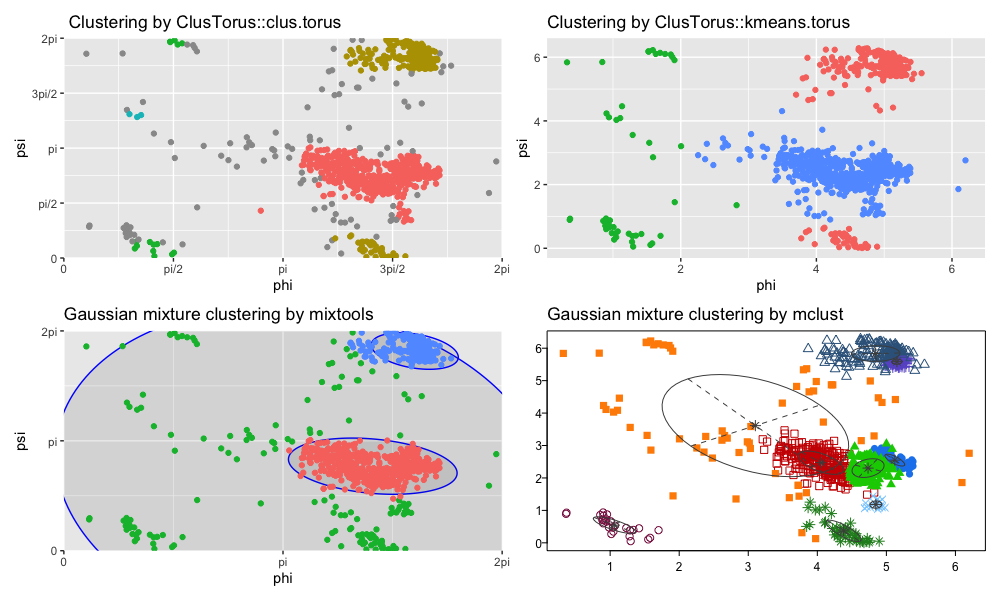
\includegraphics[scale = 0.39]{covid19.png}
     \caption{Several clustering results on Ramachandran plot for SARS-CoV-2 by using \code{clus.torus} (top left) and \code{kmeans.torus} (top right), both implemented in \CRANpkg{ClusTorus}, \code{mixtools::mvnormalmixEM} (bottom left), in which the number of components 3 is prespecified, and \code{mclust::Mclust} (bottom right), in which the number of components is chosen by BIC. Gray points in the top-left panel are ``outliers", automatically assigned by \code{clus.torus}.}
     \label{fig:covid}
 \end{figure}

 We introduce the R package \CRANpkg{ClusTorus} \citep{ClusTorus} which provides various tools for handling and clustering multivariate angular data on the torus. The package provides angular adaptations of usual clustering methods such as the $k$-means clustering and  pairwise angular distances, which can be used as an input for distance-based clustering algorithms, and implements a novel clustering method based on conformal prediction framework \citep{Vovk}. Also implemented in the package are the EM algorithms and an elliptical $k$-means algorithm for fitting mixture models on the torus, and a kernel density estimation. We will introduce various clustering tools implemented in the package, explaining choices in conformal prediction using two sets of example data. We also present the theoretical and technical background, and demonstrate these tools with R codes.

 For data on the torus, there are a few previous works for mixture modeling and clustering. \citet{Mardia:2007} proposed a mixture of bivariate von Mises distributions for data on $\mathbb{T}^2$, with an application to modeling protein backbone chain angles. \citet{Mardia:2012} proposed a density estimation on the torus, based on a mixture of approximated von Mises sine distributions, for higher dimensional cases, but the proposed EM algorithm tends to be unstable when sample sizes are limited. The R package \CRANpkg{BAMBI} \citep{Chakraborty:2019,BAMBI} provides routines to fit such von Mises mixture models using MCMC, but is only applicable to bivariate (and univariate) angles in $\mathbb{T}^2$. We have implemented EM algorithms (for $p=2$) and the elliptical $k$-means algorithm (for any $p$), originally proposed for vector-valued data \citep{Sung:1998,Bishop,Shin:2019}, for fitting mixture models on the torus. To the best of authors' knowledge, \pkg{ClusTorus} is the first implementation of methods for fitting mixture models on multidimensional tori of any dimension. 

 Algorithmic clustering for data on the torus has also been proposed. For example,
 %\citet{Kountouris:2009} proposed a predictive clustering algorithm on the torus based on a multi-class support vector machine.
 \citet{Gao:2018} used an extrinsic $k$-means algorithm for clustering protein angles. While this algorithm is not always satisfactory, it is implemented in \pkg{ClusTorus} for a quick-and-dirty analysis. The top right panel of Figure \ref{fig:covid} depicts the result of applying this algorithm with $k = 3$. Note that the popular R packages \CRANpkg{mixtools} \citep{mixtools} and \CRANpkg{mclust} \citep{mclust} provide misleading clustering results, when applied to data on the torus.  As we illustrate in Figure \ref{fig:covid}, these tools do not take into account the cyclic nature of the angular data.

 The main contribution of \pkg{ClusTorus} is an implementation of
%In addition to the above contributions for analyzing data on the torus, we adopt and implement
the predictive clustering approaches of \citet{Jung:2021} and \citet{Shin:2019}. For this, the conformal prediction framework of \citet{Vovk} is extended for multivariate angular data. The conformal prediction is a distribution-free method of constructing prediction sets, and our implementation uses kernel density estimates and mixture models, both based on the multivariate von Mises distribution \citep{Mardia:2012}.
Furthermore, by using Gaussian-like approximations of the von Mises distributions and a graph-theoretic approach,
flexible clusters, composed of unions of ellipsoids on $\mathbb{T}^p$, can be identified. %The methods implemented in \pkg{ClusTorus} are natural extensions of the $p = 2$ treatment of \citet{Jung:2021}, enabling a predictive clustering of data on $\mathbb{T}^p, p > 2$.
The proposed predictive clustering can be  obtained by simply using \code{clus.torus} as follows.
 \begin{example}
library(ClusTorus)
set.seed(2021)
ex <- clus.torus(SARS_CoV_2)
plot(ex)
 \end{example}
 The result of the predictive clustering is visualized in the top left panel of Figure~\ref{fig:covid}, which is generated by \code{plot(ex)}.  The dataset \code{SARS\_CoV\_2}, included in \pkg{ClusTorus},  collects the dihedral angles $\phi,\psi$ in the  backbone chain B of SARS-CoV-2 spike glycoprotein. The raw coronavirus protein data are available at Protein Data Back with id  6VXX \citep{Walls:2020}, and can be retrieved by using R package \pkg{bio3d}. %The unit of these angles is degrees in $\left[0^\circ,360^\circ\right)$.
 The function \code{clus.torus} performs three core procedures---conformal prediction, hyperparameter selection and cluster assignment---for predictive clustering.

The rest of this article focuses on introducing the three core procedures: (i) the conformal prediction framework, including our choices of the conformity scores, (ii) hyperparameter selection and (iii) cluster assignment. After demonstrating how the package \pkg{ClusTorus} can be used for clustering of $\mathbb{T}^2$- and $\mathbb{T}^4$-valued data, we describe how the main function \code{clus.torus} and other clustering algorithms such as $k$-means and hierarchical clustering can be used to analyze data
%, and the other clustering algorithms, including the extrinsic and the elliptical $k$-means algorithm, adapted for data
on the torus.
In the Appendix, we provide technical details and options in fitting mixture models on the torus, and a list of S3 classes defined in \pkg{ClusTorus}. 

\section{Conformal prediction}

The conformal prediction framework \citep{Vovk} is one of the main ingredients of our development. Based on the work of \citet{Vovk} and \citet{Lei:2013, Lei:2015}, we briefly introduce the basic concepts and properties of conformal prediction. Suppose that we observe a sample of size $n$, $X_i\sim F$ where $X_i\in \mathbb{T}^p$ for each $i$ and that the sequence $\mathbb{X}_n =\left\{X_1,\cdots,X_n\right\}$ is \dfn{exchangeable}. Then, for a new $X_{n+1}\sim F$, the prediction set $C_n = C_n\left(\mathbb{X}_n\right)$ is said to be valid at level $1-\alpha$ if:
\begin{align}\label{eq:1}
    P\left(X_{n+1}\in C_n\right)\ge 1-\alpha,\quad \alpha\in \left(0,1\right),
\end{align}
where $P$ is the corresponding probability measure for $\mathbb{X}_{n+1}=\mathbb{X}_n\cup\left\{X_{n+1}\right\}$.

For a given $x\in \mathbb{T}^p$, write $\mathbb{X}_{n}(x)=\mathbb{X}_n\cup\left\{x\right\}$. Consider the null hypothesis $H_0: X_{n+1}=x$, where $X_{n+1}\sim F$. To test the hypothesis, the conformal prediction framework uses \dfn{conformity scores} $\sigma_i$ defined as follows:
\begin{align*}
    \sigma_i\left(x\right) &:= g\left(X_i, \mathbb{X}_{n}\left(x\right)\right),~ \forall i=1,\cdots,n+1,\\
    \sigma\left(x\right) &:=g\left(x, \mathbb{X}_{n}\left(x\right)\right) = \sigma_{n+1}\left(x\right),
\end{align*}
for some real valued function $g$, which measures the conformity or similarity of a point to the given set. If $X_{\left(1\right)},\cdots,X_{\left(n+1\right)}$ are ordered to satisfy $\sigma_{\left(1\right)}\le\cdots\le\sigma_{\left(n+1\right)}$ for $\sigma_{\left(i\right)} = g\left(X_{\left(i\right)}, \mathbb{X}_{n+1}\right)$, then we may say that $X_{\left(n+1\right)}$ is the most similar point to $\mathbb{X}_{n+1}$.

Consider the following quantity:
\begin{align*}
    \pi\left(x\right) = \frac{1}{n+1}\sum_{i=1}^{n+1}I\left(\sigma_i\left(x\right)\le\sigma_{n+1}\left(x\right)\right),\quad I(A) = \begin{cases}
    1,\quad A\text{ is true,}\\ 0,\quad \text{otherwise,}
    \end{cases}
\end{align*}
which can be understood as a p-value for the null hypothesis $H_0$. The \dfn{conformal prediction set} of level $1-\alpha$ is constructed as
\begin{align}
    C^{\alpha}_n=\left\{x:\pi\left(x\right)>\alpha\right\}.
\end{align}
Because the sequence $\mathbb{X}_n(x)$ is exchangeable under $H_0$, $\pi\left(x\right)$ is uniformly distributed on $\left\{\frac{1}{n+1},\cdots,1\right\}$. With this property, it can be shown that the conformal prediction set is valid for finite samples, i.e., \eqref{eq:1} holds with $C_n$ replaced by $C_n^{\alpha}$ for any $F$, that is, the prediction set is distribution-free \citep{Lei:2013}. The performance of the conformal prediction highly depends on the choice of conformity score $\sigma$. In some previous works on conformal prediction \citep{Lei:2013, Lei:2015, Shin:2019, Jung:2021}, the quality of prediction sets using density based conformity scores has been satisfactory.

We demonstrate a construction of the conformal prediction set with a kernel density estimate-based conformity score, defined later in \eqref{eq:6}, for the data shown in Figure \ref{fig:covid}.
%This dataset \code{SARS\_CoV\_2} is included in \pkg{ClusTorus}. In the codes below, we pre-process the data {\color{red}by} extracting the bivariate angles in chain B only.
With the conformity score given by \eqref{eq:6}, \code{cp.torus.kde} computes the conformal prediction set $C_n^\alpha$ at a given level $1-\alpha$ ($\alpha=0.1$ below), by performing the kernel density estimation. The function tests the inclusion in $C_n^\alpha$ of each point $(\phi,\psi)$ over a fine grid of $\mathbb{T}^2$, and the result of the testing is shown as the boolean indices in the column \code{Cn} of the output below.
%
%The inclusion in $C_n^\alpha$ of each grid point can be checked with the boolean index indicated in the column \code{Cn} of the output (see below).
The columns \code{Lminus} and \code{Lplus} provide approximated prediction sets, defined in \citet{Jung:2021}.

\begin{example}
cp.kde <- cp.torus.kde(SARS_CoV_2)
cp.kde

Conformal prediction sets (Lminus, Cn, Lplus) based on kde with concentration 25

Testing inclusion to the conformal prediction set with level = 0.1 :
-------------
          phi psi Lminus    Cn Lplus level
1  0.00000000   0  FALSE FALSE FALSE   0.1
2  0.06346652   0  FALSE FALSE FALSE   0.1
3  0.12693304   0  FALSE FALSE FALSE   0.1
4  0.19039955   0  FALSE FALSE FALSE   0.1
5  0.25386607   0  FALSE FALSE FALSE   0.1
6  0.31733259   0  FALSE FALSE FALSE   0.1
7  0.38079911   0  FALSE FALSE FALSE   0.1
8  0.44426563   0  FALSE FALSE FALSE   0.1
9  0.50773215   0  FALSE FALSE FALSE   0.1
10 0.57119866   0  FALSE FALSE FALSE   0.1

 9990 rows are omitted.
\end{example}


The concentration parameter $\kappa$ of the kernel density estimation and the level(s) of the prediction set can be designated by providing arguments \code{concentration} and \code{level}. By default, these values are set as \code{concentration = 25} and \code{level = 0.1}.
%If a finer grid is needed, the argument \code{eval.point} of \code{cp.torus.kde},

%These evaluation points can be designated via the parameter \code{eval.point}
%, and testing the inclusion in $C_n^\alpha$ of the prespecified evaluation points. The evaluation points can be designated via the parameter \code{eval.point}. The function \code{grid.torus} generates a grid for the evaluation points with size \code{grid.size} on $[0,2\pi)^p$.
%The inclusion in $C_n^\alpha$ of each grid point can be checked with the boolean index indicated in the column \code{Cn} of the output (see below). The columns \code{Lminus} and \code{Lplus} provides the approximations of $C_n^\alpha$, discussed in \citet{Jung:2021}.


The output \code{cp.kde} is an S3 object with class \code{cp.torus.kde}, for which a generic method \code{plot} is available. The conformal prediction set for \code{SARS\_CoV\_2} data can be displayed on the Ramachandran plot, as follows. The result is shown in Figure \ref{fig:cpkde}.


\begin{example}
plot(cp.kde)
\end{example}

 \begin{figure}
     \centering
     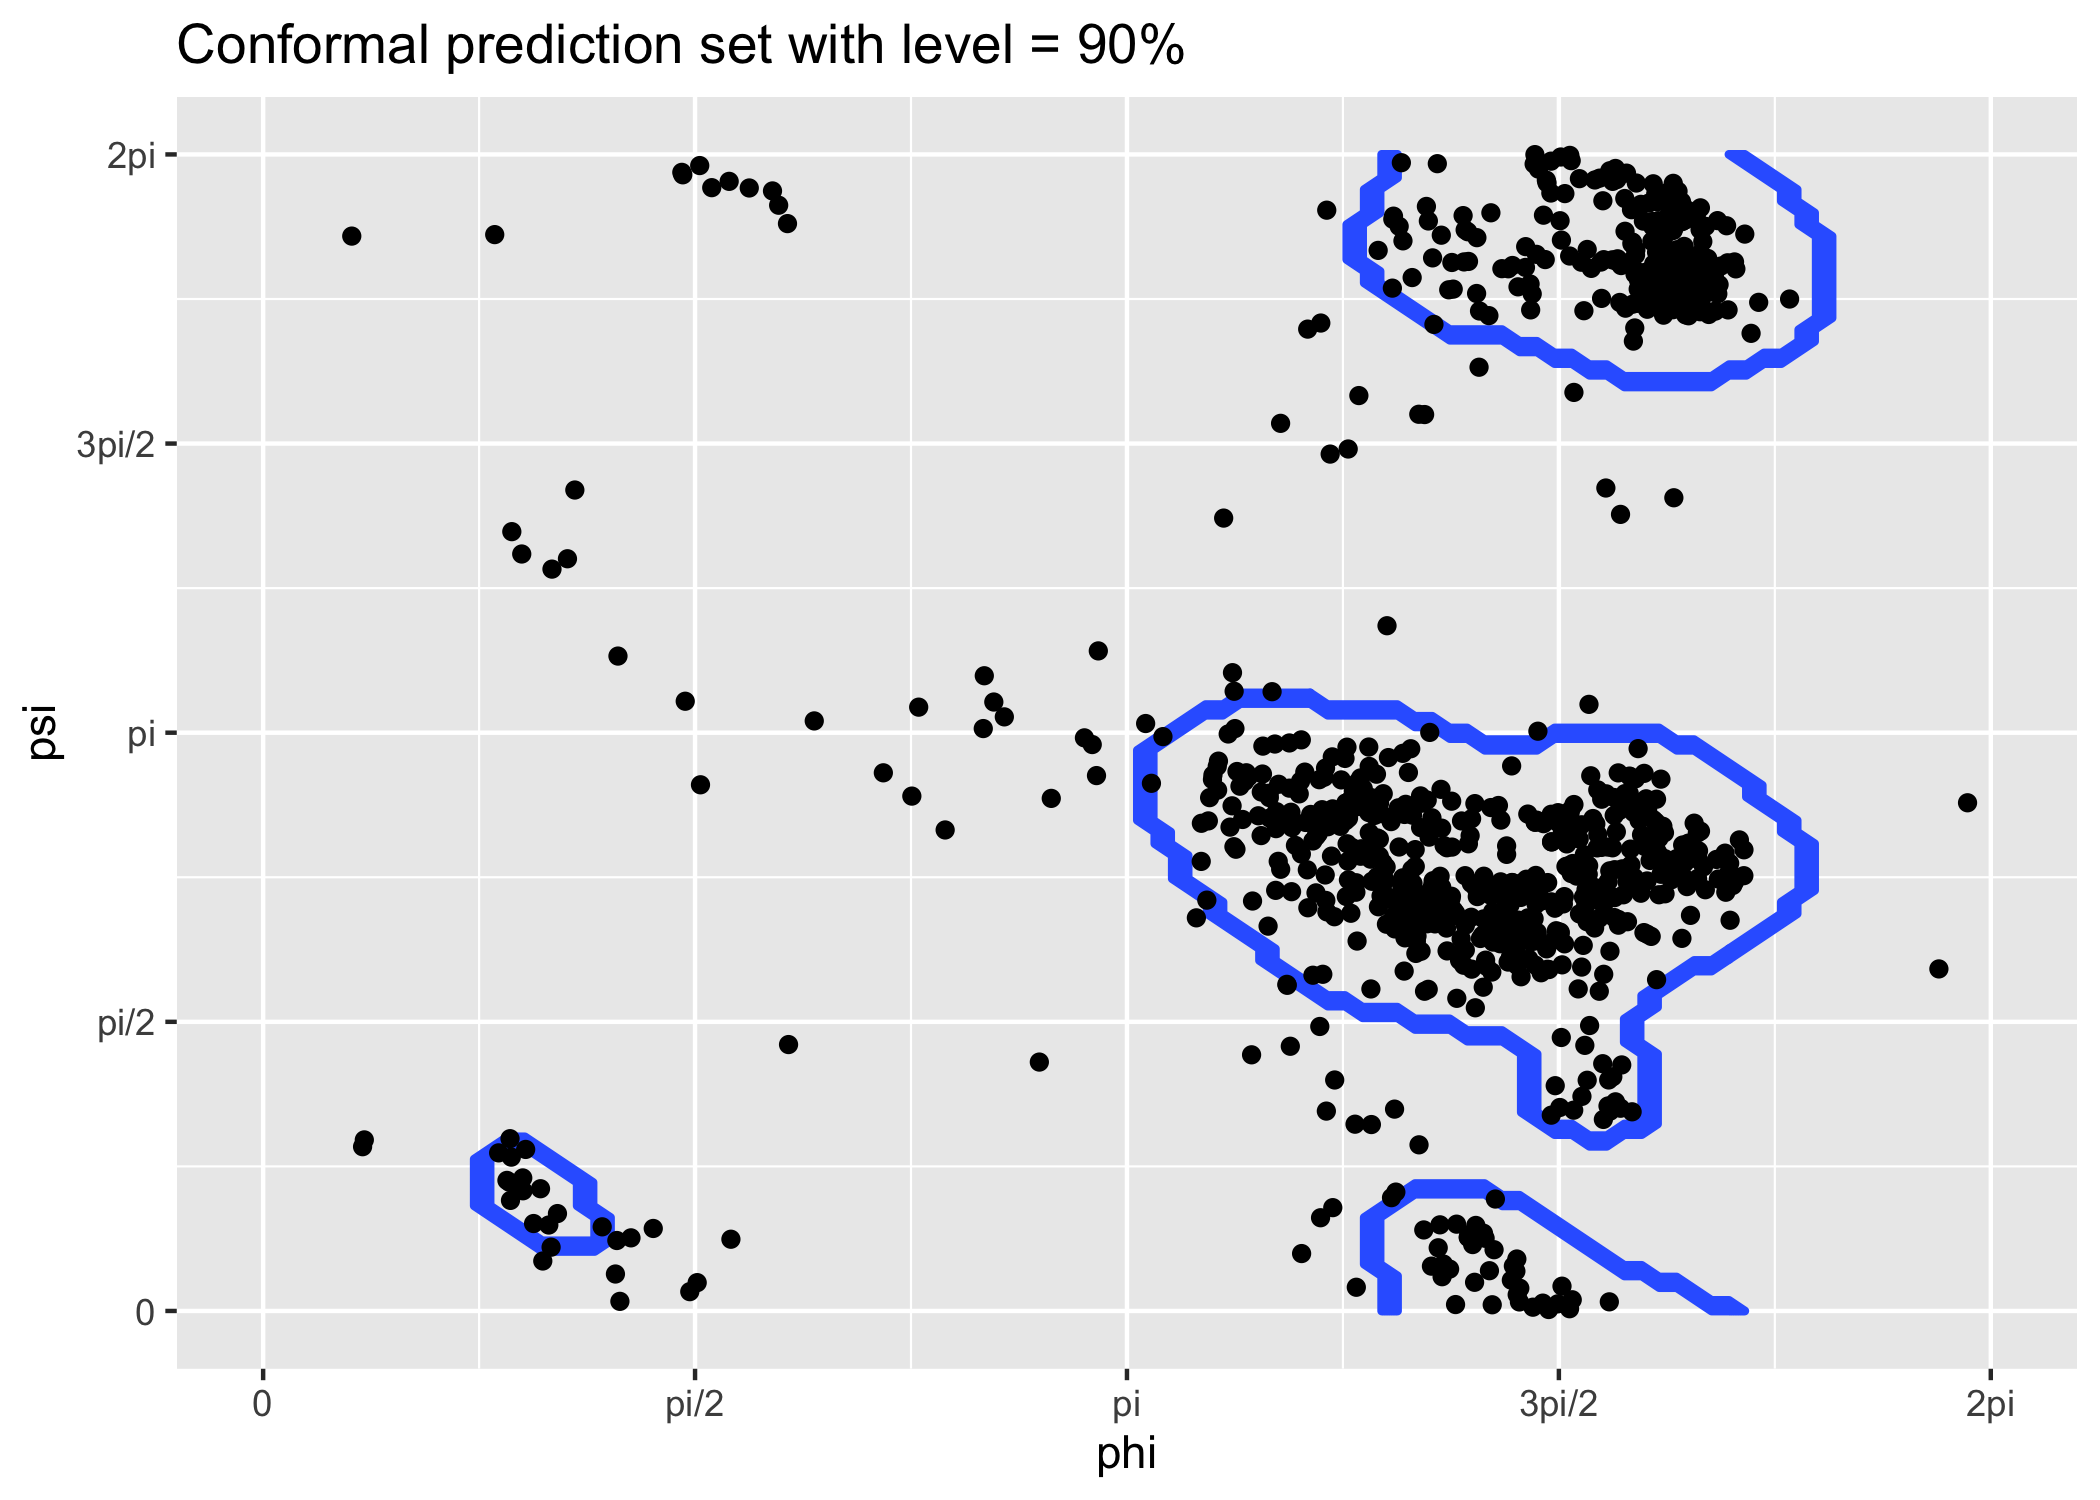
\includegraphics[scale = 0.15]{cpkde.png}
     \caption{The Ramachandran plot for SARS-CoV-2, with boundaries of the conformal prediction set,  whose conformity score is \eqref{eq:6} with $\kappa = 25$ for level $1-\alpha = 0.9$. }
     \label{fig:cpkde}
 \end{figure}

\subsection{Inductive conformal prediction}
If the sample size $n$ and the number $N$ of grid points over $\mathbb{T}^p$ are large, evaluating $n + N$ conformity scores may take a long time. That is, constructing the conformal prediction set suffers from high computational costs. A workaround for this inefficiency is \dfn{inductive conformal prediction}, which enjoys significantly lower computational cost. The inductive conformal prediction framework is based on splitting the data into two sets. The algorithm for inductive conformal prediction is given in Algorithm \ref{inductive conformal prediction}.

\begin{algorithm}
\caption{Inductive Conformal Prediction}\label{inductive conformal prediction}
\begin{algorithmic}[1]
\Procedure{inductive conformal prediction}{$\left\{X_1,\cdots,X_n\right\}, \alpha, n_1 < n$}
  \State Split the data randomly into  $\mathbb{X}_1=\left\{X_1,\cdots, X_{n_1}\right\}$, $\mathbb{X}_2=\left\{X_{n_1+1},\cdots, X_{n}\right\}$.
  \State Construct $\sigma$ with $\sigma\left(x\right) = g\left(x,\mathbb{X}_1\right)$ for some function $g$.
  \State Put $\sigma_i = g\left(X_{n_1+i},\mathbb{X}_1\right)$ and order as $\sigma_{\left(1\right)}\le\cdots\le\sigma_{\left(n_2\right)}$, where $n_2=n-n_1$.
  \State Construct $\hat{C}^{\alpha}_n = \left\{x:\sigma(x)\ge\sigma_{\left(i_{n_2,\alpha}\right)}\right\}$ where $i_{n,\alpha} = \lfloor\left(n+1\right)\alpha\rfloor$.
\EndProcedure
\end{algorithmic}
\end{algorithm}

While the sizes $n_1$ and $n_2$ of two split data sets can be of any size, they are typically set as equal sizes.
It is well-known that the output $\hat{C}^\alpha_n$ of the algorithm also satisfies the distribution-free finite-sample validity \citep{Vovk, Lei:2015}.  For fast computation, the inductive conformal prediction is primarily used in constructing prediction sets and clustering, in our implementation of \pkg{ClusTorus}. Specifically, \code{icp.torus} implements Algorithm \ref{inductive conformal prediction} for several prespecified conformity scores. As already mentioned, we need to choose the conformity score $\sigma$ carefully for better clustering performances.

Before we discuss our choices of the conformity scores, we first illustrate how the functions in \pkg{ClusTorus} are used to produce inductive conformal prediction sets. The following codes show a calculation of the inductive conformal prediction set for the data \code{SARS\_CoV\_2}. The conformal prediction set with the conformity score given by kernel density estimates \eqref{eq:6} can be constructed by \code{icp.torus} and \code{icp.torus.eval}. The function \code{icp.torus} computes $\sigma_i$'s in line 4 of Algorithm \ref{inductive conformal prediction} and \code{icp.torus.eval} tests whether pre-specified evaluation points are included in $\hat{C}_n^\alpha$. If these evaluation points are not supplied, then \code{icp.torus.eval} creates a grid of size $100 \times 100$ (for $p = 2$). % as done in \code{cp.torus.kde}.


\begin{example}
set.seed(2021)
icp.torus.kde <- icp.torus(SARS_CoV_2, model = "kde", concentration = 25)
icp.kde <- icp.torus.eval(icp.torus.kde, level = 0.1)
icp.kde

Conformal prediction set (Chat_kde)

Testing inclusion to the conformal prediction set with level = 0.1:
-------------
           X1 X2 inclusion
1  0.00000000  0     FALSE
2  0.06346652  0     FALSE
3  0.12693304  0     FALSE
4  0.19039955  0     FALSE
5  0.25386607  0     FALSE
6  0.31733259  0     FALSE
7  0.38079911  0     FALSE
8  0.44426563  0     FALSE
9  0.50773215  0     FALSE
10 0.57119866  0     FALSE

 9990 rows are omitted.
\end{example}

In the codes above, the data splitting for \code{icp.torus} is done internally, and can be inspected by
\code{icp.torus.kde\$split.id}.

%The column \code{Chat\_kde} in the output \code{icp.kde} indicates whether or not each evaluation point is in $\hat{C}_n^\alpha$.

We now introduce our choices for the conformity score $\sigma$ in the next two subsections.

\subsection{Conformity score from kernel density estimates}

For the 2-dimensional case, \citet{Jung:2021} proposed to use the kernel density estimate based on the von Mises kernel \citep{Marzio:2011} for the conformity score. A natural extension to the $p$-dimensional tori, for $p\ge 2$, is
\begin{align}\label{eq:6}
    g\left(u, \mathbb{X}_{n}\left(x\right)\right) = \frac{1}{n+1}\sum_{i=1}^{n+1}K_\kappa\left(u-X_i\right),\quad K_\kappa\left(v\right) = \prod_{i=1}^p\frac{e^{\kappa\cos\left(v_i\right)}}{2\pi I_0\left(\kappa\right)},\quad v = \left(v_1,\cdots,v_p\right)^T\in\mathbb{T}^p
\end{align}
where $I_0$ is the modified Bessel function of the first kind of order 0, and $\kappa$ is a prespecified concentration parameter. The function \code{kde.torus} provides the multivariate von Mises kernel density estimation. For conformal prediction, we take $\sigma\left(x_i\right) = g\left(x_i,\mathbb{X}_n\left(x\right)\right)$, and for inductive conformal prediction, we take $\sigma\left(x\right) = g\left(x,\mathbb{X}_1\right)$. %Note that the product von Mises kernel ensures that kernel density estimate \eqref{eq:6} is a density function of $\mathbb{T}^p$, a characteristic other choices of kernels do not possess.

\subsection{Conformity scores from mixtures of multivariate von Mises}

Our next choices of conformity scores are based on mixture models. Since the multivariate normal distributions are not defined on $\mathbb{T}^p$, we instead use the multivariate von Mises distribution \citep{Mardia:2008}, whose density on $\mathbb{T}^p$ is
\begin{align}\label{eq:7}
f\left(y;\mu,\kappa, \Lambda\right) = C\left(\kappa,\Lambda\right)\exp\left\{-\frac{1}{2}\left[\kappa^T\left(2 - 2c\left(y,\mu\right)\right)+s\left(y,\mu\right)^T\Lambda s\left(y,\mu\right)\right]\right\}
\end{align}
where $y = \left(y_1,\cdots,y_p\right)^T  \in\mathbb{T}^p$, $\mu = \left(\mu_1,\cdots,\mu_p\right)^T \in\mathbb{T}^p$, ${\kappa} = (\kappa_1,\ldots,\kappa_p)^T \in (0,\infty)^p$, $\Lambda = (\lambda_{j,l})$  for $1\le j,l \le p$, $-\infty < \lambda_{jl} < \infty$,
\begin{align*}
    c\left(y,\mu\right) &= \left(\cos\left(y_1-\mu_1\right),\cdots, \cos\left(y_p-\mu_p\right)\right)^T,\\
    s\left(y,\mu\right) &= \left(\sin\left(y_1-\mu_1\right),\cdots, \sin\left(y_p-\mu_p\right)\right)^T,\\
    \left(\Lambda\right)_{jl}&=\lambda_{jl}=\lambda_{lj},~j\ne l,\quad \left(\Lambda\right)_{jj}=\lambda_{jj}=0,
\end{align*}
and for some normalizing constant $C\left(\kappa,\Lambda\right)>0$. We write $f\left(y;\theta\right) = f\left(y;\mu,\kappa,\Lambda\right)$ for $\theta = (\mu,\kappa,\Lambda)$.

For any positive integer $J$ and a mixing probability $\boldsymbol{\pi} = \left(\pi_1,\cdots,\pi_J\right)$, consider a $J$-mixture model:
\begin{align}\label{eq:8}
    p\left(u;\boldsymbol{\pi},\boldsymbol{\theta}\right) = \sum_{j=1}^J\pi_jf\left(u;\theta_j\right)
\end{align}
where $\boldsymbol{\theta} = \left(\theta_1,\cdots,\theta_J\right)$, $\theta_j = (\mu_{j}, \kappa_{j}, \Lambda_j)$ for $j=1,\cdots,J$. Let $\left(\hat{\boldsymbol{\pi}}, \hat{\boldsymbol{\theta}}\right)$ be appropriate estimators of $\left(\boldsymbol{\pi}, \boldsymbol{\theta}\right)$ based on $\mathbb{X}_1$. The plug-in density estimate based on \eqref{eq:8} is then
\begin{align}\label{eq:9}
    p\left(\cdot;\hat{\boldsymbol{\pi}},\hat{\boldsymbol{\theta}}\right) = \sum_{j=1}^J\hat{\pi}_jf\left(\cdot;\hat{\theta}_j\right),
\end{align}
which can be used as a conformity score by setting $g\left(\cdot,\mathbb{X}_1\right)=\hat{p}\left(\cdot\right)$. Assuming high concentrations, an alternative conformity score can be set as $g\left(\cdot,\mathbb{X}_1\right)=p^{max}\left(\cdot,\hat{\boldsymbol{\pi}},\hat{\boldsymbol{\theta}}\right)$ where
\begin{align}\label{eq:10}
     p^{max}\left(u;\hat{\boldsymbol{\pi}},\hat{\boldsymbol{\theta}}\right):=\max_{j=1,\cdots,J}\left(\hat{\pi}_jf\left(u;\hat{\theta}_j\right)\right)\approx p\left(u;\hat{\boldsymbol{\pi}},\hat{\boldsymbol{\theta}}\right).
\end{align}

On the other hand, \citet{Mardia:2012} introduced an approximated density function $f^*$ for the $p$-variate von Mises sine distribution \eqref{eq:7} for sufficiently high concentrations and when $\Sigma\succ0$:
\begin{align}\notag
f^*\left(y;,\mu,\Sigma\right) = \left(2\pi\right)^{-p/2}\left|\Sigma\right|^{-1/2}\exp\left\{-\frac{1}{2}\left[\kappa^T\left(2 - 2c\left(y,\mu\right)\right)+s\left(y,\mu\right)^T\Lambda s\left(y,\mu\right)\right]\right\}
\end{align}
where $\left(\Sigma^{-1}\right)_{jl} = \lambda_{jl}, \left(\Sigma^{-1}\right)_{jj} = \kappa_j, ~j\ne l$. By further approximating via $\theta \approx \sin\theta$, $1-\frac{\theta^2}{2}\approx\cos\theta$, we write
\begin{align}
    f^*\left(y;,\mu,\Sigma\right) \approx \left(2\pi\right)^{-p/2}\left|\Sigma\right|^{-1/2}\exp\left\{-\frac{1}{2}\left[\left(y\ominus\mu\right)^T\Sigma^{-1}\left(y\ominus\mu\right)\right]\right\},\label{eq:11}
\end{align}
where the angular subtraction $\ominus$ stands for
\begin{align}\notag
X\ominus Y := \left(\arg\left(e^{i\left(\phi_{x1} - \phi_{y1}\right)}\right), \cdots, \arg\left(e^{i\left(\phi_{xp} - \phi_{yp}\right)}\right)\right)^T,
\end{align}
for $X = \left(\phi_{x1},\cdots,\phi_{xp}\right)^T\in\mathbb{T}^p$ and $Y = \left(\phi_{y1},\cdots,\phi_{yp}\right)^T\in\mathbb{T}^p$ as defined in \citet{Jung:2021} for $p = 2$. By replacing the von Mises density $f$ in \eqref{eq:10} with the approximate normal density \eqref{eq:11}, $\log\left(p^{max}\left(\cdot;\boldsymbol{\pi},\boldsymbol{\theta}\right)\right)$ is approximated by
\begin{align}
    \log\left(p^{max}\left(u;\boldsymbol{\pi},\boldsymbol{\theta}\right)\right) &\approx \frac{1}{2}\max_j e\left(u;\pi_j,\theta_j\right) + c, \nonumber\\
    e\left(u;\pi_j,\theta_j\right)&=-\left(u\ominus\mu_j\right)^T\Sigma_j^{-1}\left(u\ominus\mu_j\right) +2\log\pi_j-\log\left|\Sigma_j\right| \label{eq:ehatj}
\end{align}
where $\theta_j=(\mu_{j},\Sigma_j)$, $\mu_j = (\mu_{1j},\cdots,\mu_{pj})^T\in\mathbb{T}^p$, $\Sigma_j\in\mathbb{R}^{p\times p}$ and a constant $c\in\mathbb{R}$. Our last choice of the conformity score is
\begin{align}\label{eq:12}
g\left(\cdot,\mathbb{X}_{1}\right)=\max_je\left(\cdot,\hat{\pi}_j,\hat{\theta}_j\right).
\end{align}
Note that with this choice of conformity score, the conformal prediction set can be expressed as the union of ellipsoids on the torus. That is, the following equalities are satisfied \citep{Shin:2019, Jung:2021}: Let $C_n^e$ be the level $1-\alpha$ prediction set using \eqref{eq:12}. Then
\begin{align}\notag
    C^e_n&:=\left\{x\in\mathbb{T}^p:g\left(x,\mathbb{X}_{1}\right)\ge g\left(X_{\left(i_{n_2,\alpha}\right)},\mathbb{X}_{1}\right)\right\}\\\label{eq:14}
    &=\bigcup_{j=1}^J\hat{E}_j\left(\sigma_{\left(i_{n_2,\alpha}\right)}\right)
\end{align}
where $\hat{E}_j\left(t\right)=\left\{x\in\mathbb{T}^p:\left(x\ominus\hat{\mu}_j\right)^T\hat{\Sigma}_j^{-1}\left(x\ominus\hat{\mu}_j\right)\le 2\log\hat{\pi}_j-\log\left|\hat{\Sigma}_j\right| - t\right\}$ for $t\in\mathbb{R}$. Note that $\hat{E}_j\left(t\right)$ is automatically vanished if $t\ge 2\log\hat{\pi}_j-\log\left|\hat{\Sigma}_j\right|$.



\subsection{Implementation}

We have implemented four conformity scores,  described in the previous section. These are based on
\begin{enumerate}
    \item kernel density estimate \eqref{eq:6},
    \item mixture model \eqref{eq:9},
    \item max-mixture model \eqref{eq:10}, and
    \item ellipsoids obtained by approximating the max-mixture \eqref{eq:12}.
\end{enumerate}
The function \code{icp.torus} in \pkg{ClusTorus} computes these conformity scores using the inductive conformal prediction framework, and returns \code{icp.torus} object(s). Table \ref{table:icp.torus.score} illustrates several important arguments of the function \code{icp.torus}.

\renewcommand{\arraystretch}{1.1}
\begin{table}[hbt!]
\small
\begin{tabularx}{\textwidth}{lX}
\toprule
Arguments        & Descriptions\\ \hline
\code{data}             & $n \times d$ matrix of toroidal data on $[0, 2\pi)^d$ or $[-\pi, \pi)^d$ \\ \hline
\code{model}           & A string. One of "kde", "mixture", and "kmeans" which determines the model or estimation methods. If "kde", the model is based on the kernel density estimates. It supports the kde-based conformity score only. If "mixture", the model is based on the von Mises mixture, fitted with an EM algorithm. It supports the von Mises mixture and its variants based conformity scores. If "kmeans", the model is also based on the von Mises mixture, but the parameter estimation is implemented with the elliptical k-means algorithm illustrated in Appendix. It supports the log-max-mixture based conformity score only. If the dimension of data space is greater than 2, only "kmeans" is supported. Default is \code{model = "kmeans"}. \\ \hline
%\code{mixturefitmethod} & A string. One of "circular", "axis-aligned", and "general" which determines the constraint of the EM fitting. Default is "axis-aligned". This argument only works for \code{model = "mixture"}. \\ \hline
%\code{kmeansfitmethod}  & A string. One of "general", ellipsoids", "heterogeneous-circular" or "homogeneous-circular". If "general", the elliptical k-means algorithm with no constraint is used. If "ellipsoids", only the one iteration of the algorithm is used. If"heterogeneous-circular", the same as above, but with the constraint that ellipsoids must be spheres. If "homogeneous-circular", the same as above but the radii of the spheres are identical. Default is "general". This argument only works for \code{model = "kmeans"}. \\ \hline
\code{J}            & A scalar or numeric vector for the number(s) of components for \code{model = c("mixture", "kmeans")}. Default is \code{J = 4}.\\ \hline
\code{concentration}           &  A scalar or numeric vector for the concentration parameter(s) for \code{model = "kde"}. Default is \code{concentration = 25}.\\ \hline
%\code{init}            & Methods for choosing initial values of "kmeans" fitting. Must be "hierarchical" or "kmeans". If "hierarchical", the initial parameters are obtained with hierarchical clustering method. If "kmeans", the initial parameters are obtained with extrinsic k-means method. Additional arguments for k-means clustering and hierarchical clustering can be designated via argument \code{...}. If no options are designated, \code{nstart=1} for \code{init="kmeans"} and \code{method="complete"} for \code{init="hierarchical"} are used. Default is "hierarchical". \\
\bottomrule
\end{tabularx}
\caption{Key arguments and descriptions for the function \code{icp.torus}}
\label{table:icp.torus.score}
\end{table}

The argument {\code{model}} of the function {\code{icp.torus}} indicates which conformity score is used. By setting {\code{model = "kde"}}, the kde-based conformity score \eqref{eq:6} is used. By setting {\code{model = "mixture"}} the mixture model \eqref{eq:9} is estimated by an EM algorithm, and conformity scores based on \eqref{eq:9}, \eqref{eq:10}, \eqref{eq:12} are all provided. Setting {\code{model = "kmeans"}} provides a mixture model fit by the elliptical $k$-means algorithm and conformity score based on \eqref{eq:12}.

 The arguments \code{J} and \code{concentration} specify the model fitting hyperparameters. To compute conformity scores based on kernel density estimate \eqref{eq:6}, one needs to specify the concentration parameter $\kappa$. Likewise, the number of mixtures, $J$, needs to be specified in order to fit the mixture model \eqref{eq:9} and the variants \eqref{eq:10} and \eqref{eq:12}. The function \code{icp.torus} takes either a single value (e.g., \code{J = 4} is the default), or a vector (e.g., \code {J = 4:30} or \code{concentration = c(25,50)}) for arguments \code{J} and \code{concentration}. If  \code{J} (or \code{concentration}) is a scalar, then \code{icp.torus} returns an \code{icp.torus} object. 
 
 On the other hand, if \code{J} (or \code{concentration}) is a numeric vector containing at least two values, then \code{icp.torus} returns a list of \code{icp.torus} objects, one for each value in \code{J}  (or \code{concentration}, respectively). Typically, the hyperparameter $J$ (or $\kappa$) is not predetermined, and one needs to choose among a set of candidates. A list of \code{icp.torus} objects, evaluated for each candidate in vector-valued \code{J} (or \code{concentration}) is required for our hyperparameter selection procedure, discussed in a later section.  
%If the hyperparameter $J$ (or $\kappa$) needs to be chosen, which is typically the case, then the \code{icp.torus} objects are evaluated for each candidate of $J$ (or $\kappa$). A list of \code{icp.torus} objects is needed for selecting hyperparameters, which will be discussed in a later section. 
%Note that vector-values inputs for \code{J} (or \code{concentration}) are primarily used when the hyperparameter needs to be chosen. }

Let us present an R code example for creating an \code{icp.torus} object, fitted with \code{model = "kmeans"} (the default value for argument \code{model}) and \code{J = 12}.

\begin{example}
set.seed(2021)
icp.torus.12 <- icp.torus(SARS_CoV_2, J = 12)
plot(icp.torus.12, level = 0.1111)
\end{example}

\begin{figure}
     \centering
     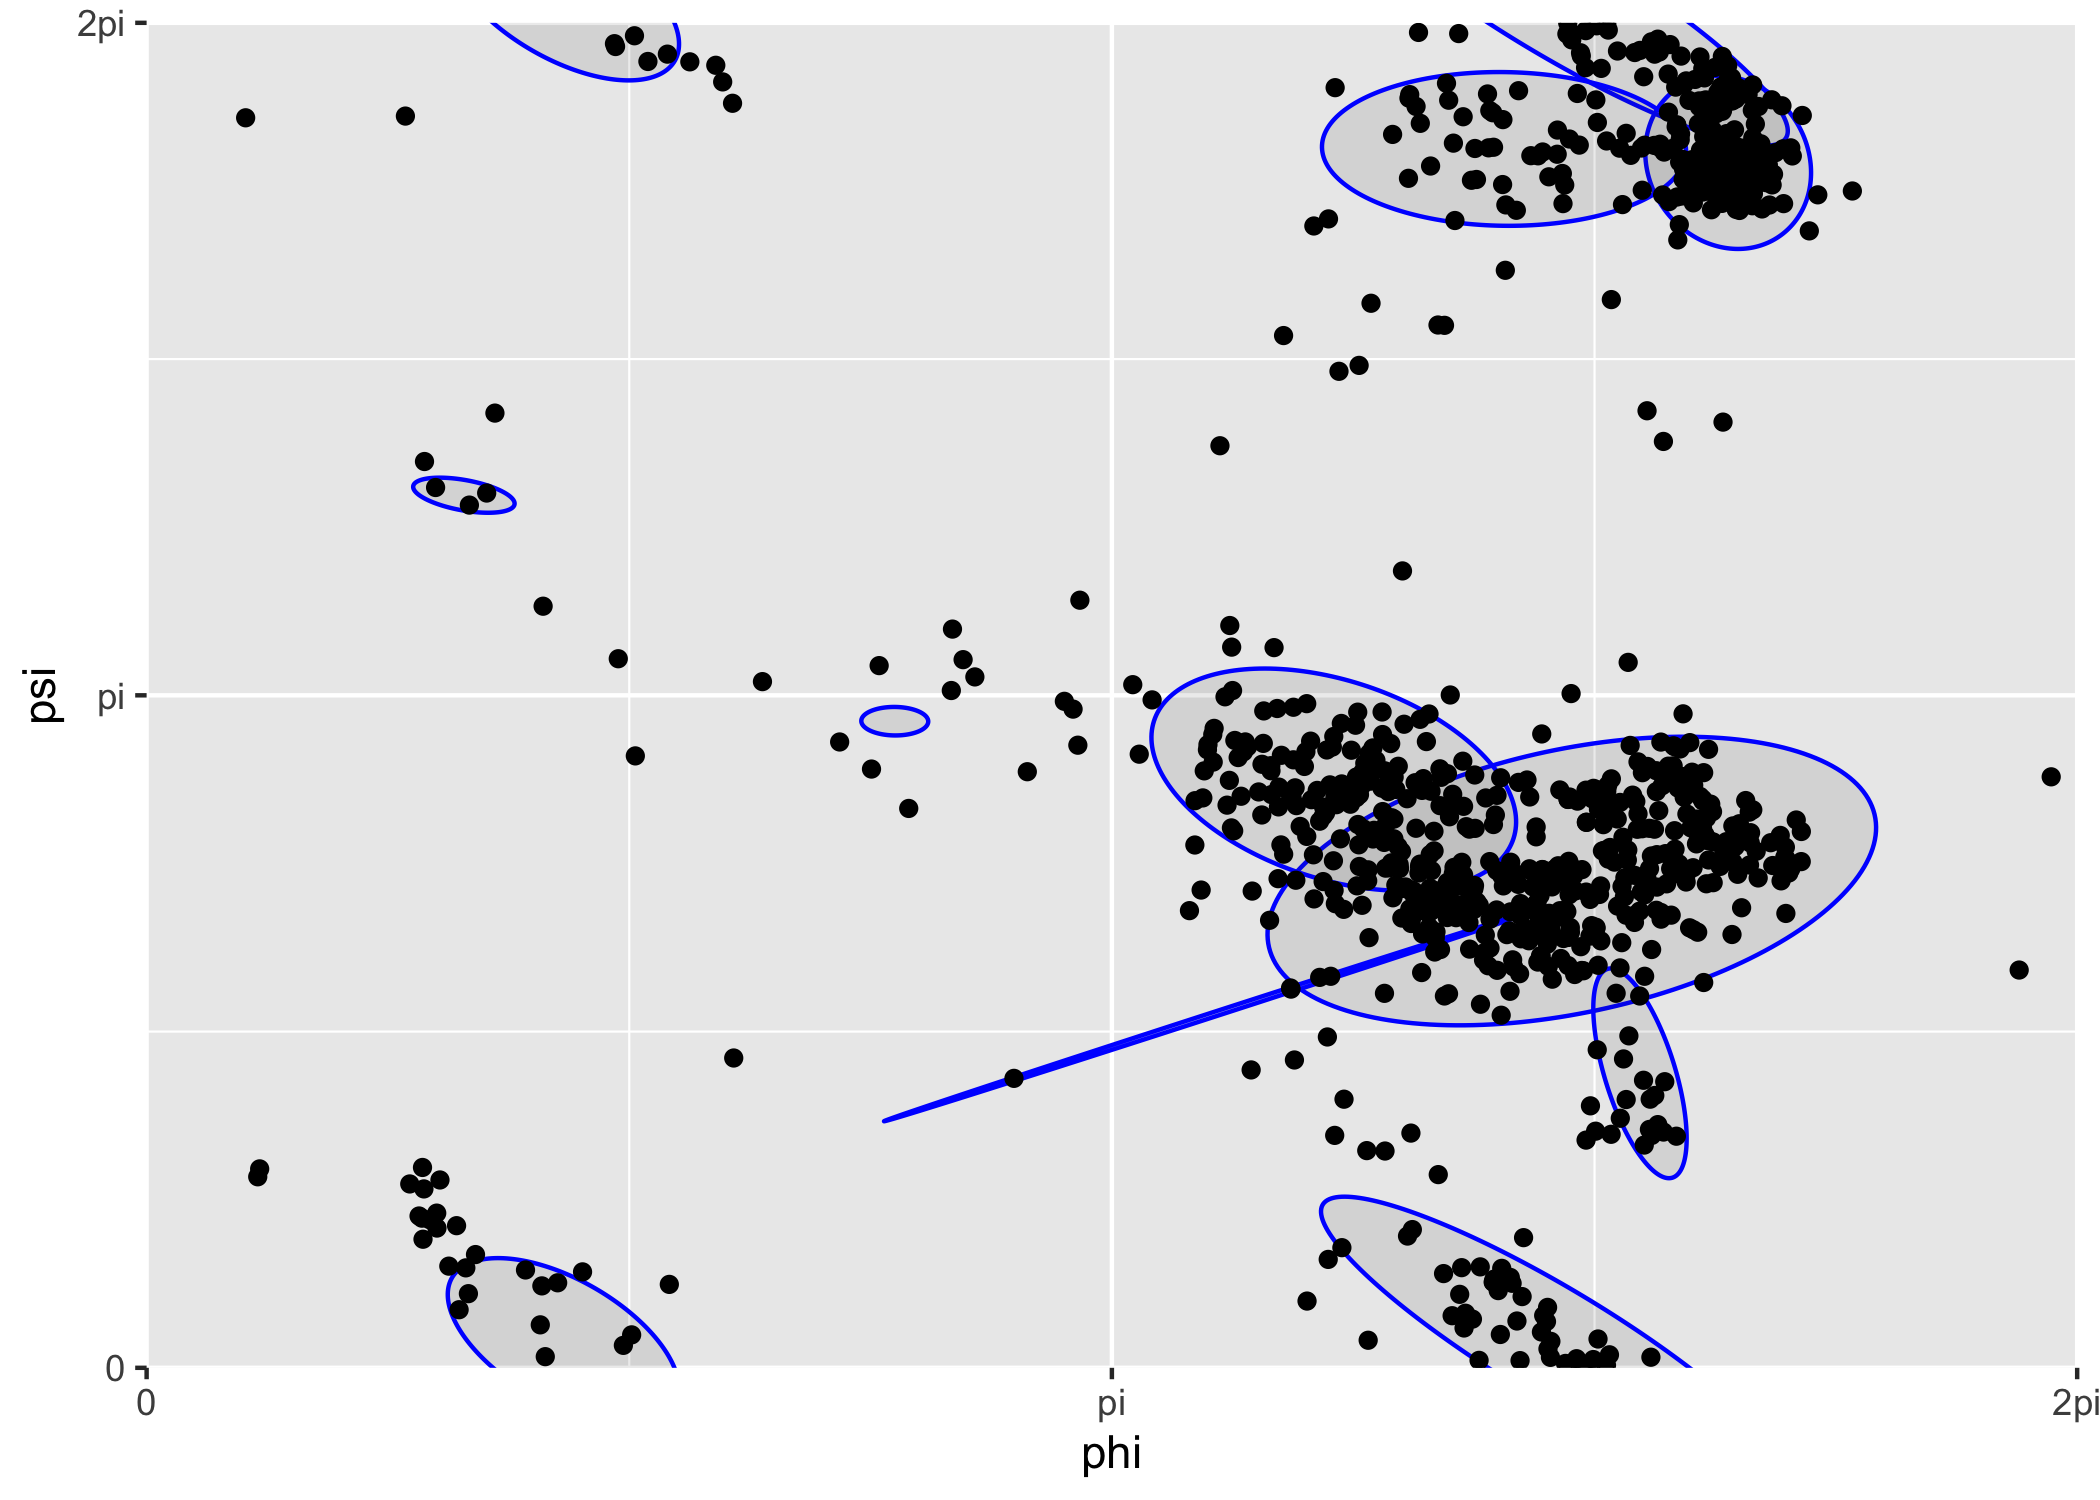
\includegraphics[scale = 0.15]{Ellipses.png}
     \caption{The Ramachandran plot for SARS-CoV-2, with conformal prediction set whose conformity score is \eqref{eq:12} with $J = 12$ for level $\alpha = 0.1111$. The plot demonstrates the union of ellipses as \eqref{eq:14}.}
     \label{fig:ellipse}
\end{figure}

 The \code{icp.torus} object has an S3 method \code{plot}, and the R code \code{plot(icp.torus.12, level = 0.1111)} plots the ellipses in \eqref{eq:14} with $\alpha$ specified by argument \code{level = 0.1111}. The union of these ellipses is in fact the inductive conformal prediction set of level $1-\alpha$. The boundaries of the inductive conformal prediction set can be displayed by specifying \code{ellipse = FALSE}, as follows. 
 \begin{example}
plot(icp.torus.12, ellipse = FALSE)
 \end{example}

The resulting graphic is omitted. 
%
%
%Figure \ref{fig:ellipse} shows that the shape of conformal prediction set is actually a union of ellipsoids, when using {\color{red}\code{icp.torus}} with {\color{red}\code{model  = "kmeans"}} and \code{kmeansfitmethod = "general"}.

%
%{\color{red}Following codes are implementation for Figure \ref{fig:ellipse} under \code{J=12} and \code{level = 0.1111}. Note that the function \code{icp.torus} generates a list of \code{icp.torus} objects, if the argument \code{J} is input with a numeric vector. The choice of \code{J=12, level = 0.1111} will be dealt later. Also note that we will use the default initialization, i.e., \code{init="hierarchical"} by passing no arguments for hierarchical clustering. That is, from now on, our code will be implemented with hierarchical clustering initialization, whose method is complete-linkage.
%\begin{example}
%> set.seed(2021)
%> icp.torus.12 <- icp.torus(SARS_CoV_2, J = 12)
%> plot(icp.torus.12, level = 0.1111)
%\end{example}
%}
 

Conformity scores based on mixture model and its variants need appropriate estimators of the parameters, $\boldsymbol{\pi}$ and $\boldsymbol{\theta}$. If the parameters are poorly estimated, the conformal prediction sets will be constructed trivially and thus become useless. We have implemented two methods of estimation: EM algorithms and the elliptical $k$-means algorithm, also known as the generalized Lloyd's algorithm \citep{Sung:1998, Bishop, Shin:2019}. EM algorithms for the mixture model \eqref{eq:9} are described in \citet{Jung:2021}, for the 2-dimensional case. Since the EM estimates require long computation time and large sample sizes, extensions to higher-dimensional tori do not seem to apt. The EM estimates of the mixture model parameters can be naturally used for the case of max-mixture \eqref{eq:10} and ellipsoids \eqref{eq:12} as well. The argument {\code{model = "mixture"}} of \code{icp.torus} works only for the 2-dimensional case. On the other hand, the elliptical $k$-means algorithm converges much faster even for moderately high-dimensional tori. The elliptical $k$-means algorithm is used for estimating parameters in the approximated normal density \eqref{eq:11}, and for computation of the conformity score of ellipsoids \eqref{eq:12}. The elliptical $k$-means algorithms for data on the torus are further discussed in the Appendix.

%The protein structure data we aim to analyze typically consist of hundreds of angles (observations). Fitting the mixture with a large number of components may give inefficient estimators. Thus, we have implemented options for reducing the number of model parameters, by constraining the shape of the ellipsoids. {\color{red} Applying the constraints lead much faster convergence for estimating parameters \citep{grim2017approximation}}. The following constraints for $\Sigma$ are the options to determine the shape of the ellipsoids.
%\begin{itemize}
%    \item $\Sigma_j=\sigma^2_jI_p$ for some $\sigma^2_j>0$ for all $j$, and the prediction set will be the union of spheres. \code{mixturefitmethod = "circular"} and \code{kmeansfitmethod = "heterogeneous-circular"} represents this constraint. Furthermore, if $\sigma^2_1 = \cdots = \sigma^2_J$ and $\pi_j = 1/J$ for all $j$, then all the spheres have the same radii and this constraint can be designated with \code{kmeansfitmethod = "homogeneous-circular"}.
 %   \item $\Sigma_j = diag\left(\sigma^2_{jk}\right)_{k=1,\cdots,p}$ for $\sigma^2_{jk}>0$, and the fitted ellipsoids $\hat{E}_j$ $(j=1,\cdots,J)$ are the axis-aligned ellipsoids. \code{mixturefitmethod = "axis-aligned"} represents this constraint.
%    \item No constraint for $\Sigma_j$, and $\hat{E}_j$ $(j=1,\cdots,J)$ are any ellipsoids. This option can be designated by \code{mixturefitmethod = "general"}, \code{kmeansfitmethod = "ellipsoids"} and \code{kmeansfitmethod = "general"}. (See Table \ref{table:icp.torus.score} for the difference between \code{kmeansfitmethod = "ellipsoids"} and \code{kmeansfitmethod = "general"}.)
%\end{itemize}

Table \ref{conformity score} summarizes the four choices of  conformity scores in terms of model-fitting methods, dimensionality of the data space, and whether clustering is available. Our predictive clustering is implemented only based on the "ellipsoids" conformity score \eqref{eq:12}. The rational for this choice is due to the relatively simple form of prediction sets (a union of ellipsoids \eqref{eq:14}). %Figure \ref{fig:ellipse} shows that the shape of conformal prediction set is actually a union of ellipsoids, when using {\color{red}\code{icp.torus}} with {\color{red}\code{model  = "kmeans"}} and \code{kmeansfitmethod = "general"}.


% Moreover, because testing the intersection of ellipsoids is a univariate root finding problem \citep{Gilitschenski:2012}, this geometric property is quite useful to generating and assigning clusters for each data point, which will be discussed in the next section. If the conformity score is not the form of \eqref{eq:12}, it is quite difficult to construct clusters due to the irregular shape of the prediction sets. In summary, the geometric properties of ellipsoids is quite useful for faster convergence and generating clusters.

\begin{table}[hbt!]
\begin{center}
\begin{tabular}{ cccccc }
\toprule
Conformity Scores & EM & k-means & dim = 2 & dim > 2 & Clustering\\
\midrule
\multirow{4}{9em}{Kernel density (\ref{eq:6}) Mixture (\ref{eq:9}) Max-mixture (\ref{eq:10}) Ellipsoids (\ref{eq:12})} &  & & \checkmark & &\\
& \checkmark & & \checkmark & &\\
& \checkmark & & \checkmark & &\\
& \checkmark & \checkmark & \checkmark & \checkmark & \checkmark \\
\bottomrule
\end{tabular}
\caption{Conformity scores against available fitting methods, dimensions of the torus, and whether cluster assignment is available. }
\label{conformity score}
\end{center}
\end{table}


\section{Clustering by conformal prediction}

We now describe our clustering strategies using the conformal prediction sets. Suppose for now that the level $\alpha$ and the hyperparameter $J$ of the prediction set are given. The basic idea of clustering is to take each connected component of the prediction set as a cluster. For this, we need an algorithm identifying connected components from any prediction set. Since the prediction sets are in general of irregular shapes, such an identification is a quite difficult task. However, as shown in \citet{Jung:2021}, if the conformal prediction set is of the form \eqref{eq:14}, clusters are identified by testing the intersection of ellipsoids. Suppose $C_n^e = \cup_{j=1}^J \hat{E}_j$ where each $\hat{E}_j$ is an ellipsoid. Let the $(i,j)$th entry of a square matrix $A$ be 0 if $\hat{E}_i\cap \hat{E}_j=\varnothing$, 1 otherwise. Then, $A$ is the adjacent matrix of a graph whose nodes and edges represent the ellipsoids and intersections, respectively. The adjacent matrix $A$ gives a partition $I_1,\cdots,I_K\subseteq \{1,\cdots,J\}$ satisfying
\begin{align*}
    \hat{E}_{i_k}\cap \hat{E}_{i_{k^\prime}} = \varnothing,\quad k\ne k^\prime
\end{align*}
where $1\le k,k^\prime\le K, i_k\in I_k, i_{k^\prime}\in I_{k^\prime}$. This implies that the union of ellipsoids, $U_k=\cup_{i\in I_k}\hat{E}_i$, whose indices are in a connected component $I_k$ for some $k$, can be regarded as a cluster. That is, $U_1,\cdots,U_K$ are the disjoint clusters. With this, the conformal prediction set naturally generates $K$ clusters. Note that testing the intersection of ellipsoids can be done efficiently (which is a univariate root finding problem \citep{Gilitschenski:2012}), while testing the intersection of arbitrarily shaped sets is not feasible in general. This is the reason why we only use the conformity score of the form \eqref{eq:12}, the prediction set from which is exactly the union of ellipsoids.

We now describe how the cluster labels are assigned to data points. Each data point included in the prediction set is automatically assigned to the cluster which contains the point. For the data points which are not included in the conformal prediction set, we have implemented two different types for cluster assignment, as defined in \citet{Jung:2021}.
 The first is to assign the \emph{closest} cluster label. The notion of closest cluster can be defined either by the Mahalanobis distance $(x\ominus\hat\mu_j)^T\hat\Sigma_j^{-1}(x\ominus\hat\mu_j)$,  the approximate log-density (\ref{eq:ehatj}), or the largest posterior probability $\hat{P}(Y = k | X = x)$. For example, for $x\not\in C^e_n$, let $E_i$ be the set with the largest approximate log-density $\hat{e}_i(x)$. If $i\in I_k$, then $x$ is assigned to the cluster $k$. These provide three choices of cluster assignment,  depending on the definition of ``closeness." 
%One choice is to assign the closest cluster label. For $x\not\in C^e_n$, let $E_i$ be the set closest to $x$, in terms of the Mahalanobis distance. If $i\in I_k$, then $x$ is assigned to the cluster $k$.
The last choice is to regard the excluded points as outliers.  That is, if $x\not\in C^e_n$, then the point $x$ is labeled as ``outlier." This outlier-disposing clustering may be more appropriate for the cases where some of data points are truely outliers. Figure \ref{fig:mahal} compares the two different types of clustering assignment.

\begin{figure}
     \centering
     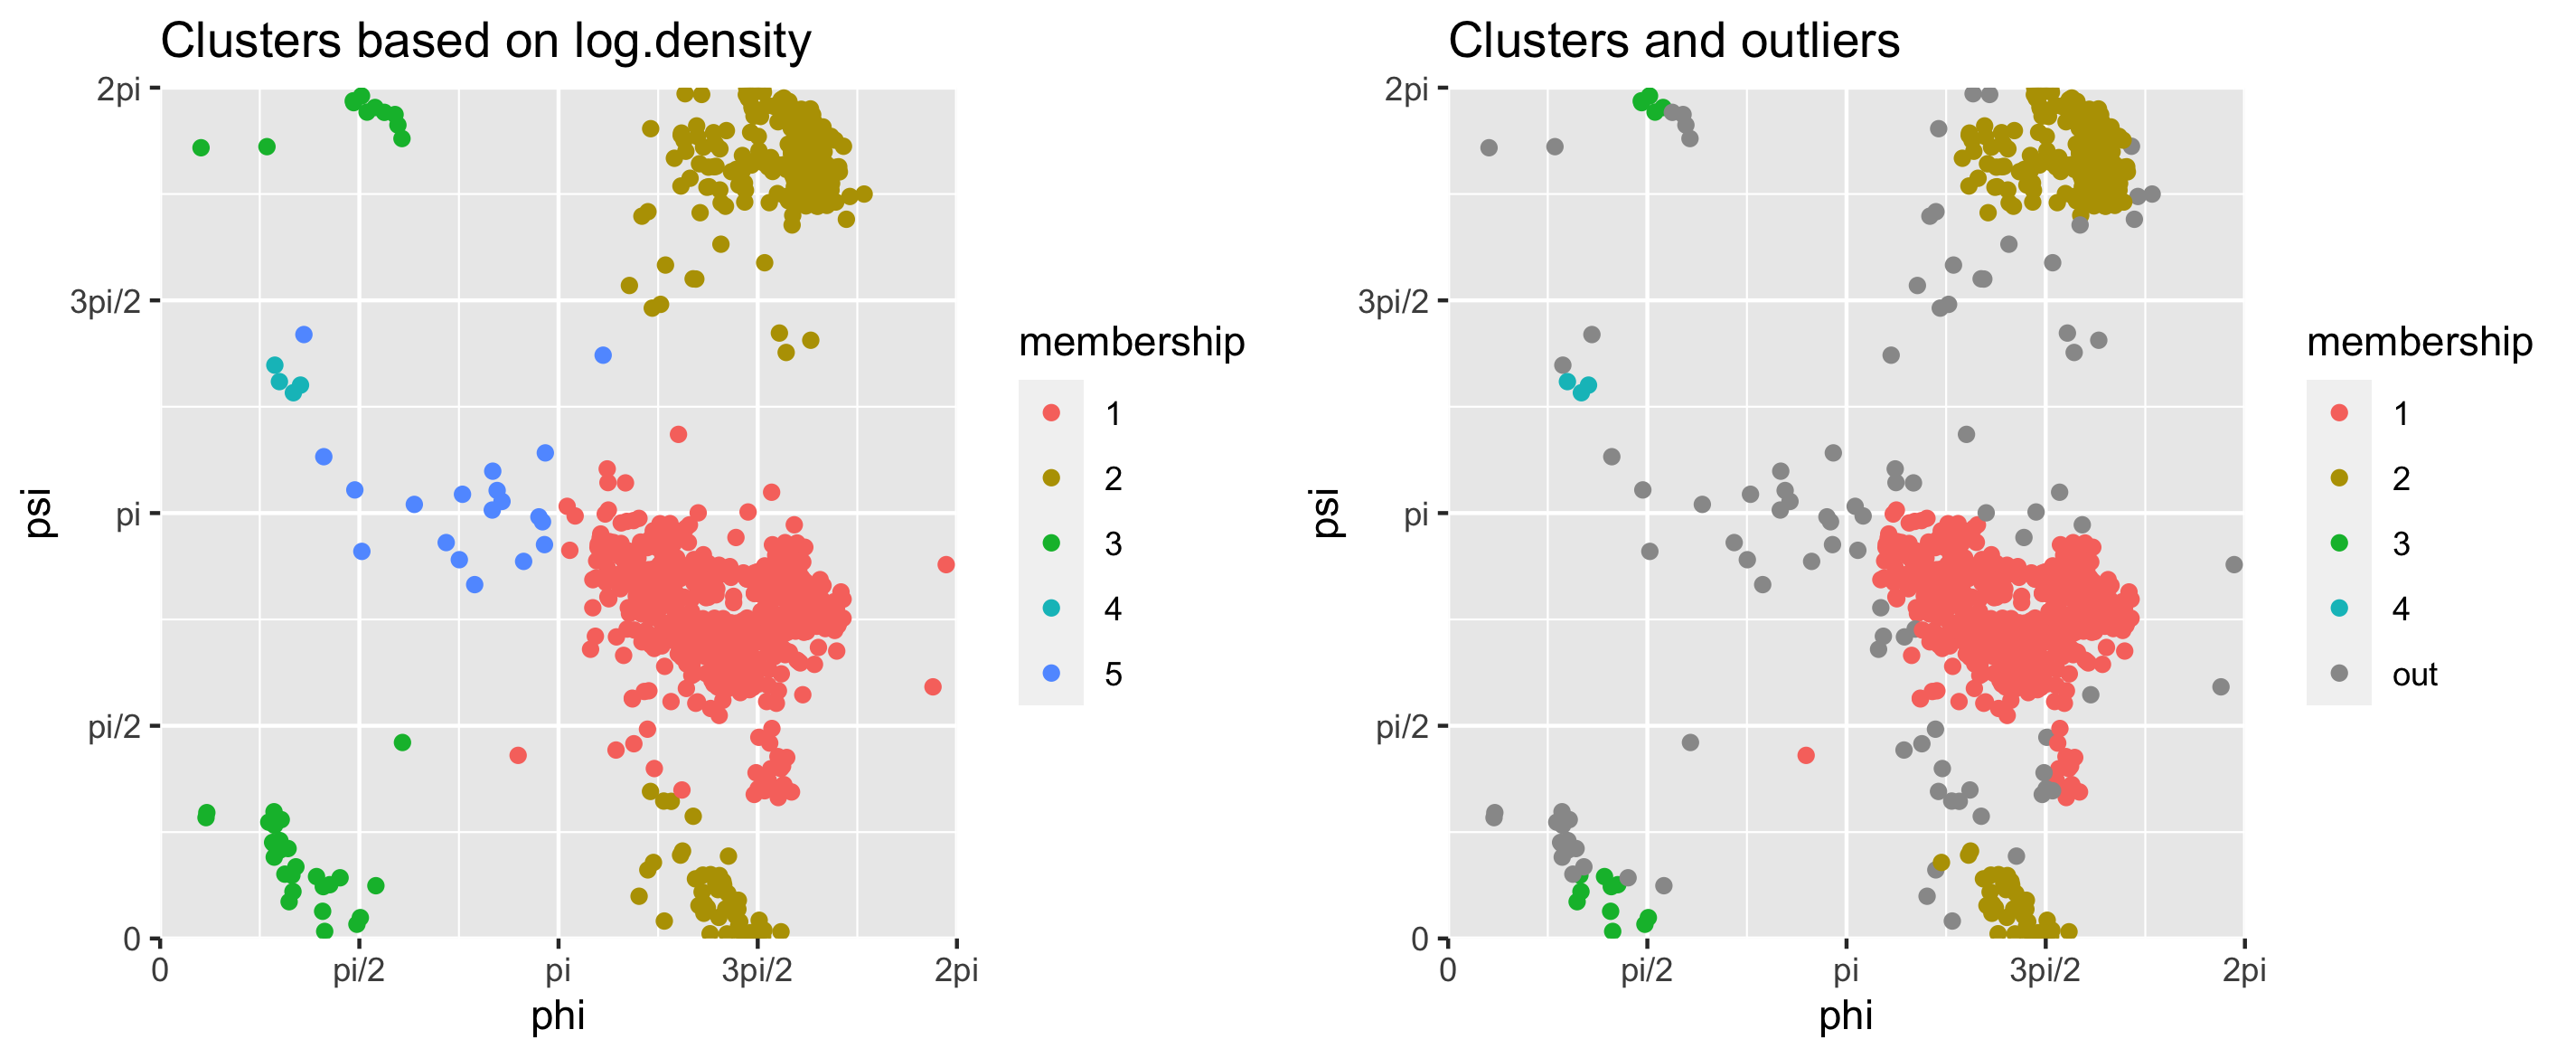
\includegraphics[scale = 0.13]{mahal.png}
     \caption{1 }
     \label{fig:mahal}
\end{figure}

The function \code{cluster.assign.torus}, which takes as input an \code{icp.torus} object and \code{level} $\alpha$, generates the clusters as we described above. The output of the function is an S3 object with class \code{cluter.obj}, and includes the cluster memberships of all data points, for each and every cluster assignment method we discussed above. 
%Since our parameter fitting method was \code{method = "kmeans"} in the object \code{icp.torus}, we can check the membership of each data point by inspecting \code{\$kmeans\$cluster.id.by.ehat} and \code{\$kmeans\$cluster.id.outlier}, which represents the results of distance clustering and outlier disposing clustering repsectively. 
The output of \code{cluster.assign.torus} includes the number of clusters detected, the cluster assignment results for the first 10 observations, and cluster sizes, as shown in the code example below.

\begin{example}
c <- cluster.assign.torus(icp.torus.12, level = 0.1111)
c

Number of clusters: 5
-------------
Clustering results by log density:
 [1] 1 1 1 1 2 4 2 1 3 1
cluster sizes: 538 372 39 4 19

Clustering results by posterior:
 [1] 5 5 5 5 2 4 3 5 3 5
cluster sizes: 6 310 104 4 548

Clustering results by representing outliers:
 [1] 1 1 1 1 2 6 2 1 6 1
cluster sizes: 508 343 15 3 0 103

 Note: cluster id = 6 represents outliers.

Clustering results by Mahalanobis distance:
 [1] 1 1 1 1 2 4 2 1 3 1
cluster sizes: 533 372 39 4 24

962 clustering results are omitted.
\end{example}


The clustering results contained in the object \code{c} can be visualized as follows.  

\begin{example}
plot(c, assignment = "log.density")
plot(c, assignment = "outlier")
\end{example}

The results are displayed in Figure \ref{fig:mahal}. When the argument \code{assignment} is not specified, the outlier disposing assignment is chosen by default. 

%In the above, $J = 12$ and $\alpha = 0.1111$. See the next section for the choice of $J$ and $\alpha$ and for how \code{icp.torus} was generated. Note that \code{c\$cluster.id.outlier} has the $6$th cluster, which actually indicates that the data point is the outlier.

\section{Hyperparameter selection}

Poor choices of conformity score result in too wide prediction sets. Thus, we need to choose the hyperparameters elaborately for a better conformal prediction set and for a better clustering performance.  The hyperparameters are the concentration parameter $\kappa$ (for the case \eqref{eq:6}) or the number of mixture components $J$ (for the cases \eqref{eq:9}, \eqref{eq:10}, \eqref{eq:12}), as well as the level $\alpha$ for all cases. There have been some efforts to select the optimal hyperparameters by introducing adequate criteria. \citet{Lei:2013} and \citet{Jung:2021} each proposed criteria based on the minimum volume of the conformal prediction set. However, as we shall see, these approaches become computationally infeasible for higher dimensions.

We briefly review the criterion used in \citet{Jung:2021}. Assume for now that mixture models are used; that is, $(J, \alpha)$ are the hyperparameters of interest.  For a set $C\subseteq\mathbb{T}^p$, let $\mu(C)$ be the volume of $C$. Without loss of generality, we can assume that $\mu\left(\mathbb{T}^p\right)=1$. For a given level $\alpha$, the optimal choice of hyperparameter $J$ minimizes $\mu\left(C_n(\alpha,J)\right)$ of conformal prediction set $C_n\left(\alpha, J\right)$. To choose $\alpha$ and $J$ altogether, \citet{Jung:2021} proposed to use the following criterion:
\begin{align}\label{eq:16}
\left(\hat{\alpha},\hat{J}\right) = \arg\min_{\alpha, J}\alpha + \mu\left(C_n\left(\alpha, J\right)\right).
\end{align}
Note that if $(\kappa, \alpha)$ are the hyperparameters, then $J$ and $\hat{J}$ in  \eqref{eq:16} are replaced by $\kappa$ and $\hat\kappa$. 

 To evaluate \eqref{eq:16}, one needs to have a set of candidates for $J$ (or $\kappa$), and conformal prediction sets corresponding to each choice of $J$ (or $\kappa$, respectively). For this purpose, the function \code{icp.torus} is designed to take as input a set of hyperparameter candidates. As an example, the following code evaluates the inductive conformal prediction sets for data \code{SARS\_CoV\_2}, fitted by mixture models with the number of components given by each $J = 3,4,\ldots, 35$.
  
\begin{example}
set.seed(2021)
icp.torus.objects <- icp.torus(SARS_CoV_2, J = 3:35)
\end{example} 

The result, \code{icp.torus.objects}, is a list of 33 \code{icp.torus} objects. Evaluating \citet{Jung:2021}'s criterion \eqref{eq:16} is implemented in the function \code{hyperparam.torus}. There, the criterion \eqref{eq:16} is termed "elbow", since the minimizer $(\hat\alpha,\hat{J})$ is typically found at an elbow of the graph of the objective function. 

\begin{example}
hyperparam.out <- hyperparam.torus(icp.torus.objects)
hyperparam.out

Type of conformity score: kmeans general
Optimizing method: elbow
-------------
Optimally chosen parameters. Number of components =  12 , alpha =  0.1111111
Results based on criterion elbow :
      J     alpha     mu criterion
2241 12 0.1111111 0.1215 0.2326111
2244 12 0.1172840 0.1169 0.2341840
2242 12 0.1131687 0.1211 0.2342687
2243 12 0.1152263 0.1198 0.2350263
2001 11 0.1172840 0.1179 0.2351840
2240 12 0.1090535 0.1265 0.2355535
2245 12 0.1193416 0.1169 0.2362416
2002 11 0.1193416 0.1175 0.2368416
2494 13 0.1316872 0.1053 0.2369872
2004 11 0.1234568 0.1136 0.2370568
2246 12 0.1213992 0.1161 0.2374992
2003 11 0.1213992 0.1163 0.2376992
2005 11 0.1255144 0.1123 0.2378144
1999 11 0.1131687 0.1248 0.2379687
2239 12 0.1069959 0.1310 0.2379959

8004 rows are omitted.

Available components:
[1] "model"     "option"    "results"   "icp.torus" "Jhat"      "alphahat"
\end{example} 
 
It can be checked that 
 the choice of $J=12$ and $\alpha = 0.1111$ in the previous examples was indeed given by the option "elbow".
 
 

 
 
% criterion is also defined for choosing $(\kappa, \alpha)$modified for the kernel density based prediction set by considering the function $\left(\hat{\alpha},\hat{\kappa}\right) \rightarrow \alpha + \mu\left(C_n\left(\alpha, \kappa\right)\right)$.
In computing the criterion \eqref{eq:16}, the volume $\mu\left(C_n\left(\alpha, J\right)\right)$ is numerically approximated. This is feasible for data on $\mathbb{T}^2=[0,2\pi)^2$ by inspecting the inclusion of each point of a fine grid.
%
%
%Since \code{icp.torus.eval} tests the inclusion of the prespecified evaluation points, by testing sufficiently many grid points, the volume $\mu\left(C_n\left(\alpha, J\right)\right)$ is approximated. %Evaluating the criterion \eqref{eq:16} for a range of $J$ values is implemented in \code{hyperparam.torus} with \code{option = "elbow"} for mixture models.
%{\color{red} For relatively low dimensional cases, e.g. $\mathbb{T}^2$, selecting $(\alpha, J)$ or $(\alpha,\kappa)$ under this criterion is computationally feasible; even if we make a fine grid of $\mathbb{T}^2=[0,2\pi)^2$ by dividing each coordinate into 100 different points, we only need to inspect the inclusion of $100^2$ different grid points. Note that the kernel density based conformity score \eqref{eq:6} is available only for 2 dimensional cases in our implementation, as we described in Table \ref{table:icp.torus.score}. Enjoying low dimensionality, we choose the concentration $\kappa$ and the level $\alpha$ simultaneously under criterion \eqref{eq:16}.}
%
However, for high dimensional cases, for example $\mathbb{T}^4$, evaluating the volume %of a given conformal prediction set by inspecting a fine grid of $\mathbb{T}^4$ 
becomes computationally infeasible. In fact, as the dimension increases, the number of required inspections grows exponentially. Furthermore, the function {$(\alpha,J)\rightarrow \alpha + \mu\left(C_n(\alpha,J)\right)$} is typically not a convex function and has multiple local minima. Thus, the choice of $\left(\hat{\alpha},\hat{J}\right)$ by \eqref{eq:16} tends to be unstable, resulting in high variability of the clustering results. Therefore, evaluating \eqref{eq:16} is not practical for high-dimensional data.

To this end, we have developed and implemented a computationally more efficient procedure for hyperparameter selection, which also provides  more stable clustering results. This procedure is a two-step procedure, first choosing the model parameter $J$, then choosing the level $\alpha$. The two-step procedure is implemented for choosing $J$ and $\alpha$, but not for $\kappa$ and $\alpha$. %
% On the other hand, if we can choose $J$ regardless of the choice of the level $\alpha$, the computational cost can be saved compared to the jointly choosing scheme such as the criterion \eqref{eq:16}. Furthermore, for given $J$, if we can choose the most "stable" $\alpha$ in the sense of the constructed number of the clusters, the computational cost for choosing $\alpha$ only stems from testing the intersection of ellipsoids. This must be much faster than the volume based searching; for given $J$ and dimension $p$, the number of intersection tests is at most $3^p\times J(J-1)/2$, but there are $100^p$ fine grid points to test the inclusion for evaluating the volume of the prediction set. By combining them, we suggest a sequential hyperparameter selection method for the mixture based conformity scores \eqref{eq:9}, \eqref{eq:10} and \eqref{eq:12}, which chooses the number of mixture components $J$ first and then the level $\alpha$ sequentially.
Our approach is in contrast to the approaches in \citet{Lei:2013} and \citet{Shin:2019} in which they only choose the model parameter for a prespecified level $\alpha$.

The first step of the procedure is to choose $J$, without making any reference to the level $\alpha$. Choosing $J$ can be regarded as selecting an appropriate mixture model. The model selection is based on either the (prediction) risk, Akaike information criterion \citep{Akaike:1974}, or Bayesian information criterion \citep{Schwarz:1978}. Since the mixture model-based conformity scores \eqref{eq:9}, \eqref{eq:10} and \eqref{eq:12} are actually the density or the approximated log-density of the mixture model, we use the conformity scores in place of the likelihood. For example, the sum of the conformity scores \eqref{eq:12} over the given data is exactly the fitted log-likelihood. Specifically, let $\mathbb{X}_1,\mathbb{X}_2$ be the splitted datasets given by Algorithm \ref{inductive conformal prediction} and $\mathbb{X} = \mathbb{X}_1\cup\mathbb{X}_2$. Let $\sigma(\cdot) = \log g\left(\cdot;\mathbb{X}_1\right)$ if $g$ is given by \eqref{eq:9} and \eqref{eq:10} or $\sigma(\cdot) = g\left(\cdot;\mathbb{X}_1\right)$ if $g$ is given by \eqref{eq:12}. Recall that $g$ is the conformity score, and it depends on the estimated model $\hat{p}$. Then, the function $\sigma$ we defined above also depends on the model $\hat{p}$, and the criterion $R$ can be defined as follows:
\begin{align}\notag
R\left(\mathbb{X},\hat{p}\right) =
\begin{cases}
-2\sum_{x\in\mathbb{X}_2}\sigma(x) & \mbox{if the criterion is the risk,} \\
-2\sum_{x\in\mathbb{X}_1}\sigma(x) + 2k & \mbox{if the criterion is AIC,}\\
-2\sum_{x\in\mathbb{X}_1}\sigma(x) + k\log n_1 & \mbox{if the criterion is BIC,}
\end{cases}
\end{align}
where $k$ is the number of model parameters and $n_1$ is the cardinality of $\mathbb{X}_1$. The function \code{hyperparam.J} computes the minimizer $\hat{J}$ of the criterion, as summarized in Algorithm \ref{hyperparam.J}.

\begin{algorithm}[hbt!]
\caption{hyperparam.J}\label{hyperparam.J}
\begin{algorithmic}[1]
\Procedure{hyperparam.J}{$\mathbb{X}\subset\mathbb{T}^p$, fitted models $\hat{p}_{j_1},\cdots,\hat{p}_{j_n}$, criterion $R$}
  \State Evaluate $R_j = R\left(\mathbb{X},\hat{p}_j\right)$  for $j = j_1,\cdots, j_n$.
  \State Evaluate $\hat{J} = \arg\min_{j\in \{j_1,\cdots,j_n\}}R_j$.
  \State Output $\hat{J},\hat{p}_{\hat{J}}$.
\EndProcedure
\end{algorithmic}
\end{algorithm}

The fitted models $\hat{p}_{j_1},\cdots,\hat{p}_{j_n}$ of Algorithm \ref{hyperparam.J} are exactly the outputs of \code{icp.torus} for various $J=j_1,\cdots,j_n$. Which criterion to use is specified by setting the argument \code{option} of \code{hyperparam.J}. The argument \code{option = "risk"}, \code{"AIC"}, or \code{"BIC"} is for the risk, AIC, or BIC, respectively. By choosing $\hat{J}$, we also fix the model $\hat{p}_{\hat{J}}$ for the next step.

The second step is to choose the level $\alpha\in (0,1)$ for the chosen $\hat{J}$ and $\hat{p}_{\hat{J}}$, so that the clustering result is stable over perturbations of $\alpha$. If the number of clusters does not change by varying the level $\alpha\in I$ for some interval $I$, we regard that the clustering result is stable on $I$. If $I$ is sufficiently wide, it is reasonable to choose an $\alpha\in I$. Thus, our strategy is to find the most wide interval $I = [a,b]\subseteq (0,1)$ whose elements construct the same number of clusters, and to set $\hat{\alpha}$ as the midpoint of the interval, i.e. $\hat\alpha = (a+b)/2$. %This mid-point choice is for enjoying the stability. 
However, choosing $\alpha$ large, e.g. $\alpha>0.5$, results in a too small coverage $1-\alpha$ of the prediction set. Thus, we restrict the searching area as $[0, M]$ for $M\in (0,1)$ which is close to $0$, and find the desirable $I$ in the restricted area $[0,M]$ rather than the whole interval $[0,1]$. This strategy is implemented in \code{hyperparam.alpha}, and the algorithm is described in Algorithm \ref{hyperparam.alpha}.

\begin{algorithm}
\caption{hyperparam.alpha}\label{hyperparam.alpha}
\begin{algorithmic}[1]
\Procedure{hyperparam.alpha}{fitted model $\hat{p}$, $n_2 := |\mathbb{X}_2|$, $M\in [0,1]$}
  \State Evaluate the number of clusters $c_{\alpha_j}$ for $\alpha_j = j/n_{2}$,  $j=1,\cdots,\lfloor n_{2} M\rfloor$.
  \State % Insert $\alpha$ to the set $A$ if $c_{\alpha-\epsilon}\ne c_{\alpha+\epsilon}$ for sufficiently small $\epsilon>0$.
  Set $A = \{j: c_{\alpha_{j-1}}\ne c_{\alpha_j},\quad j=2,\cdots,\lfloor n_{2}M\rfloor\}$.
  \State For $A=\{\alpha_{j_1},\cdots,\alpha_{j_N}\}$ find $i=\arg\max_{k\in\{1,\cdots, N-1\}}\alpha_{j_{k+1}} - \alpha_{j_k}$.
  \State Output $\hat{\alpha} = \left(\alpha_{j_{i+1}} + \alpha_{j_i}\right)/2$
\EndProcedure
\end{algorithmic}
\end{algorithm}
Note that we could alternatively input an array of levels, for the argument \code{alphavec} of \code{hyperparam.alpha}, if there is a prespecified searching area.
% When an array of levels $\{\alpha_1,\cdots,\alpha_N\}$ with $\alpha_1<\cdots<\alpha_N$ for some $N\in\mathbb{N}$ is specified, line 3 of Algorithm \ref{hyperparam.alpha} is slightly modified: for $i\in\{2,\cdots,N\}$, insert $\alpha_i$ to the set $A$ if $c_{\alpha_{i-1}}\ne c_{\alpha_{i}}$. An array of levels can be input with argument \code{alphavec} of \code{hyperparam.alpha}.
In our experience, setting $M = 0.15$ gives generally satisfying results. By setting $M = 0.15$, at most 15\% of the data points are not included in the prediction set, and at most 15\% of the data can be regarded as the outliers. The default value for argument \code{alpha.lim} of \code{hyperparam.alpha}, which is $M$ in Algorithm \ref{hyperparam.alpha}, is 0.15. We may interpret this level selecting procedure as finding the representative modes for the given mixture model; the chosen level is the cutoff value for which the most stable modes are not vanished. 

In summary, we first choose the number of model components $J$ in view of model selection, and then find the most stable level $\hat{\alpha}$ in the sense of invariability of the number of clusters. The function \code{hyperparam.torus} combines and implements Algorithms \ref{hyperparam.J} and \ref{hyperparam.alpha} sequentially and thus chooses $J$ and $\alpha$. This two-step hyperparameter selection procedure is used when mixture models are used to produce the conformal prediction sets, and can be invoked when the argument \code{option} of \code{hyperparam.torus} is set as \code{option = "risk"}, \code{"AIC"}, or \code{"BIC"}. 
If \code{option = "elbow"} (the default value, if the dimension of data is $p  = 2$), then the "elbow" criterion \eqref{eq:16} is used to choose either $(J, \alpha)$ or $(\kappa, \alpha)$. %The function 
%
%Actually, the criterion used in \citet{Jung:2021} is also supported by setting the argument \code{option="elbow"}. 
The function \code{hyperparam.torus} returns the chosen hyperparameters $(\hat{J}, \hat\alpha)$ (or $(\hat\kappa, \hat\alpha)$), as well as the corresponding model as an \code{icp.torus} object. 

As an example, the following code applies the two-step procedure with \code{option = "risk"} to \code{icp.torus.objects} we evaluated earlier.

\begin{example}
hyperparam.risk.out <- hyperparam.torus(icp.torus.objects, option = "risk")
hyperparam.risk.out

Type of conformity score: kmeans general 
Optimizing method: risk 
-------------
Optimally chosen parameters. Number of components =  12 , alpha =  0.132716 
Results based on criterion risk :
    J criterion
1   3  2016.575
2   4  1990.566
3   5  1907.887
4   6  1922.430
5   7  1924.768
... (omitted)
\end{example}

With the option "risk," $(\hat{J}, \hat\alpha) = (12, 0.0.1327)$. 
Recall that with option "elbow", we have chosen $(\hat{J}, \hat\alpha) = (12, 0.1111)$. The hyperparameter selection procedures can be visualized by \code{plot(hyperparam.out)} and \code{plot(hyperparam.risk.out)}. (The resulting graphic is omitted.)
%
%selects the optimal hyperparameters under the prespecified criterion, and also chooses the optimal fitted model by containing \code{icp.torus} object in its outputs. 
%Table \ref{table:hyperparam.torus} summarizes key arguments and options for \code{hyperparam.torus}. 
%The codes below show an example for \code{option="elbow"} with \code{SARS\_CoV\_2} data, which chooses $J = 12$ and $\alpha = 0.1111$ for Figure \ref{fig:ellipse}. 

In the next section, the two-step procedures for hyperparameter selection are used in a cluster analysis of data on $\mathbb{T}^4$. 
%{\color{red} Utilizing the two-step procedures for hyperparameter selection is further exemplified in the next section.}

%\renewcommand{\arraystretch}{1.1}
%\begin{table}[hbt!]
%\small
%\begin{tabularx}{\textwidth}{lX}
%\toprule
%Arguments               & Descriptions \\\hline
%\code{data}             & $n \times d$ matrix of toroidal data on $[0, 2\pi)^d$ or $[-\pi, \pi)^d$ \\ \hline
%\code{icp.torus.object} & A list whose elements are \code{icp.torus} objects which are generated by {\color{red}\code{icp.torus}}.\\ \hline
%\code{option}           & A string. One of \code{"elbow"}, \code{"risk"}, \code{"AIC"}, or \code{"BIC"}, which determines the criterion for the model selection. \code{"risk"} is based on the negative log-likelihood, \code{"AIC"} for the Akaike Information Criterion, and \code{"BIC"} for the Bayesian Information Criterion. \code{"elbow"} is based on minimizing the criterion \eqref{eq:16}. {\color{red}Default is \code{option = "elbow"} for 2-dimensional cases and \code{option = "risk"} for d(>2)-dimensional cases.}\\ \hline
%\code{alpha.lim}        & A positive number lower than 1, which is the upper bound of level searching interval. Default is 0.15. \\ \hline
%\code{eval.point}       & $N \times 2$ numeric matrix on $[0, 2\pi)^2$ for \code{option="elbow"}. Default input is \code{grid.torus}, which is the function for generating grid points on $\mathbb{T}^2$.\\
%\bottomrule
%\end{tabularx}
%\caption{Key arguments and descriptions for the function \code{hyperparam.torus}}
%\label{table:hyperparam.torus}
%\end{table}

%\begin{example}
%> set.seed(2021)
%> icp.torus.objects <- icp.torus(SARS_CoV_2, J = 3:35)
%> hyperparam <- hyperparam.torus(icp.torus.objects)
%> hyperparam
%Type of conformity score: kmeans general
%Optimizing method: elbow
%-------------
%Optimally chosen parameters. Number of components =  12 , alpha =  0.1111111
%Results based on criterion elbow :
%      J     alpha     mu criterion
%2241 12 0.1111111 0.1215 0.2326111
%2244 12 0.1172840 0.1169 0.2341840
%2242 12 0.1131687 0.1211 0.2342687
%2243 12 0.1152263 0.1198 0.2350263
%2001 11 0.1172840 0.1179 0.2351840
%2240 12 0.1090535 0.1265 0.2355535
%2245 12 0.1193416 0.1169 0.2362416
%2002 11 0.1193416 0.1175 0.2368416
%2494 13 0.1316872 0.1053 0.2369872
%2004 11 0.1234568 0.1136 0.2370568
%2246 12 0.1213992 0.1161 0.2374992
%2003 11 0.1213992 0.1163 0.2376992
%2005 11 0.1255144 0.1123 0.2378144
%1999 11 0.1131687 0.1248 0.2379687
%2239 12 0.1069959 0.1310 0.2379959
%
%8004 rows are omitted.
%
%Available components:
%[1] "model"     "option"    "results"   "icp.torus" "Jhat"      "alphahat"
%\end{example}

\section{Clustering data on $\mathbb{T}^4$}

In this section, we give an example of clustering \code{ILE} data in $\mathbb{T}^4$. \code{ILE} is a dataset included in \pkg{ClusTorus}, which represents the structure of the isoleucine. This dataset is obtained by collecting several different \file{.pdb} files in the Protein Data Bank \citep{pdb}. We used PISCES \citep{pisces} to select high-quality protein data, by using several benchmarks---resolution is 1.6\AA$~$or better, R-factor is $0.22$ or better, sequence percentage identity is equal to or less than $25$---as described in \citet{Tim:2010} and \citet{Mardia:2012}. %We use several benchmarks: resolution is 1.6\AA$~$or better, R-factor is $0.22$ or better, sequence percentage identity is equal to or less than $25$. %
The \code{ILE} data consist of $n = 8080$ instances of four angles $(\phi, \psi, \chi_1,\chi_2) \in \mathbb{T}^4$, and is displayed in Figure \ref{fig:ile}. 

\begin{figure}
     \centering
     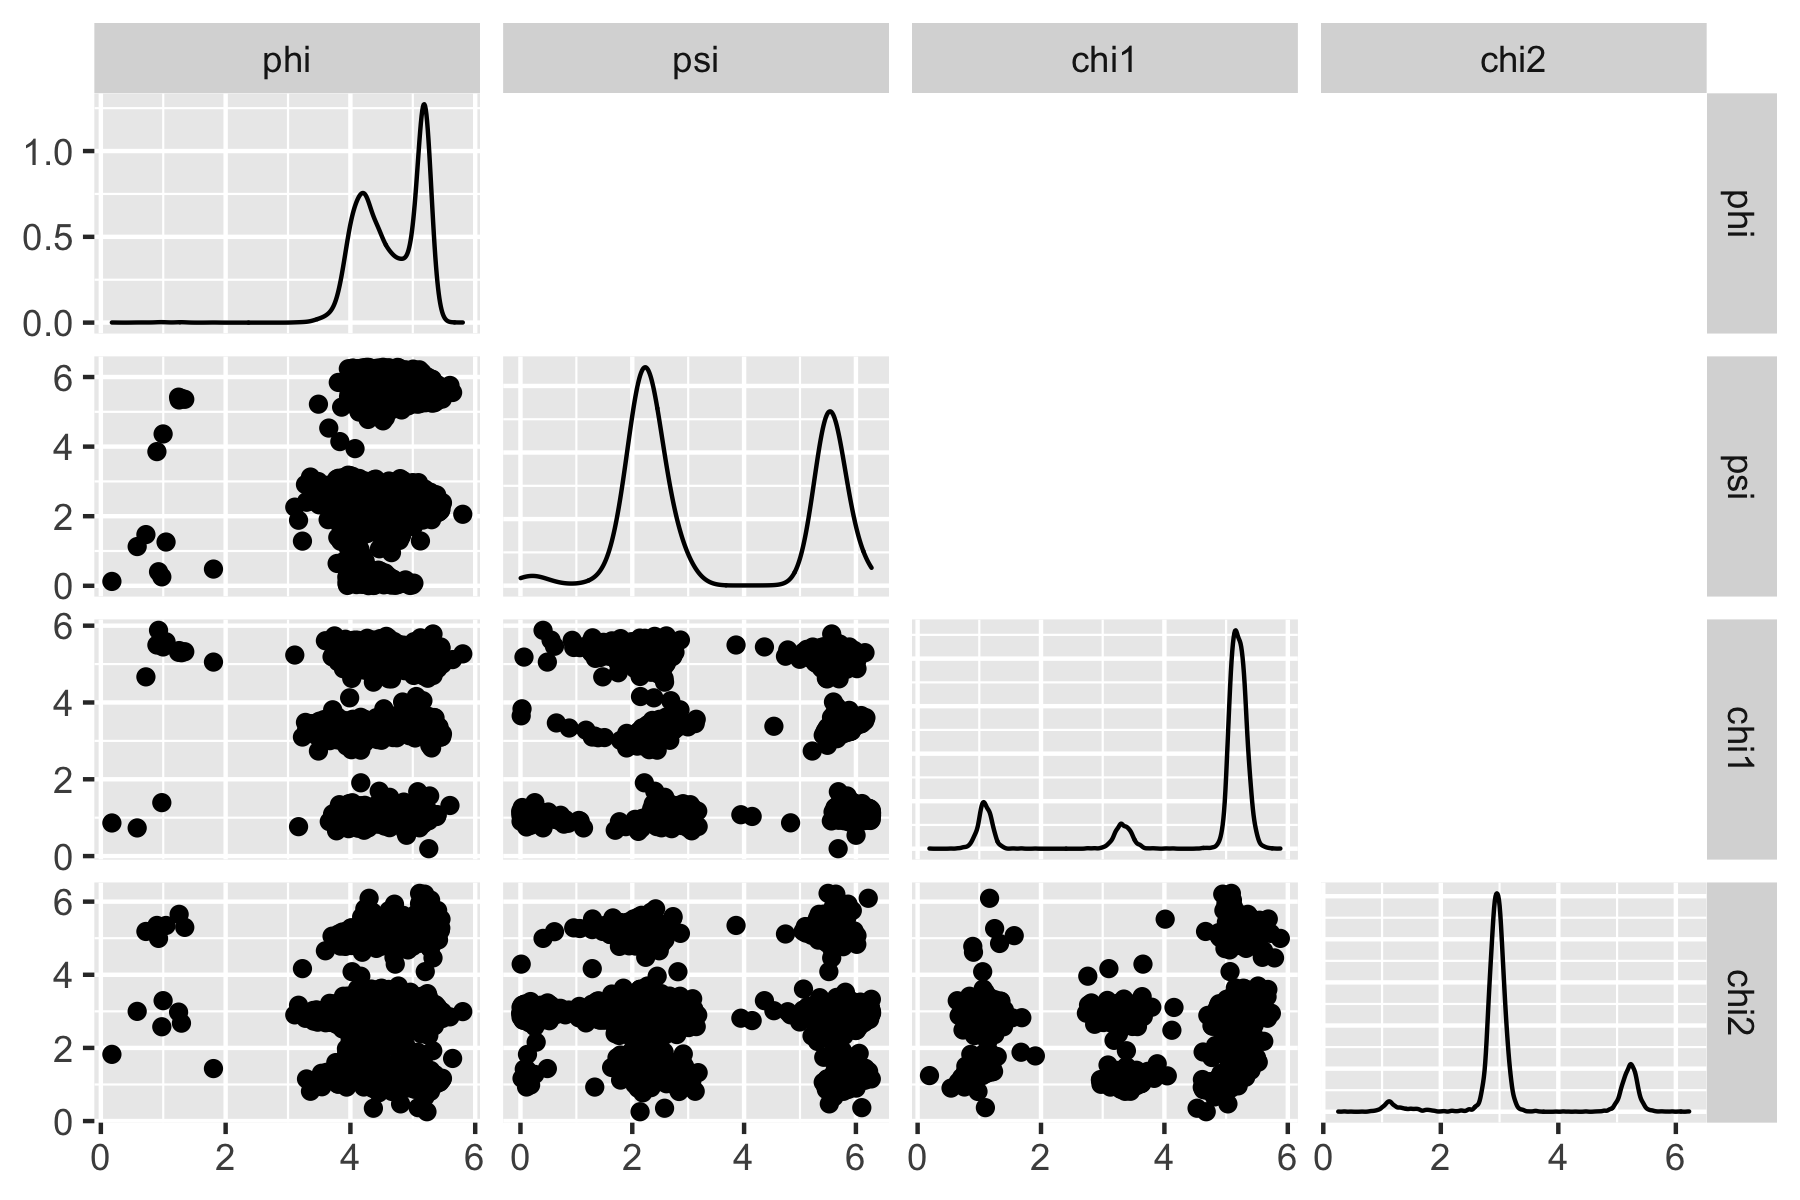
\includegraphics[scale = 0.2]{ILE.png}
     \caption{The pairwise scatter plots of \code{ILE} data, in which there are four variables (angles) $\phi,\psi,\chi_1$ and $\chi_2$. Each diagonal entry of the plot shows a marginal kernel density estimate for the corresponding angle. Each off-diagonal panel is a scatter plot for a pair of variables.}
     \label{fig:ile}
\end{figure}

For predictive clustering of \code{ILE} data, the conformal prediction sets and scores are built from mixture models, fitted with the elliptical $k$-means algorithm (i.e., \code{model = "kmeans"}). Other choices of models such as \code{"kde"} and \code{"mixture"} are not applicable for this data set with $p > 2$.
The number $J$ of components in the mixture model needs to be tuned, and we set the candidates for $J$ as $\{10,\ldots, 40\}$. In the code example below,  conformal prediction sets from mixture models are constructed  by the function \code{icp.torus}, with \code{J = 10:40} indicating the candidates of $J$.  
\begin{example}
set.seed(2021)
icp.torus.objects <- icp.torus(ILE, J = 10:40)
\end{example}

Next step is to select the hyperparameter $J$, and the level $\alpha$ of the prediction set, using the function \code{hyperparam.torus}. As discussed in the previous section, for this data set with $p = 4$, evaluating the "elbow" criterion is computationally infeasible, and is not supported in \code{hyperparam.torus}, if $p > 2$. 
For $p > 2$, \code{hyperparam.torus} uses the two-step procedure, discussed in the previous section, with \code{option = "risk"} as the default choice for the criterion. 
In the code example below, we use the two-step procedure, but apply all three available criteria (\code{option = "risk"},  \code{"AIC"}, and \code{"BIC"}) in choosing $\hat{J}$. 

\begin{example}
output_list <- sapply( c("risk", "AIC", "BIC"), function(opt) {
     hyperparam.torus(icp.torus.objects, option = opt)}, 
     simplify = FALSE,
     USE.NAMES = TRUE)
\end{example}

The result \code{output\_list} is a list of length 3, consisting of outputs of the function \code{hyperparam.torus}. The details of hyperparameter selection can be visualized, and are shown in Figure \ref{fig:criterion}. The first row of the figure is created by \code{plot(output\_list\$risk)}, and shows that the evaluated prediction risk is the smallest at $\hat{J} = 29$. On the right panel, it can be seen that the longest streak of the number of clusters over varying level $\alpha$ occurs at 16, which is given by a range of levels around $\hat\alpha = 0.1093$. The second and third rows are similarly generated, and they show the results of AIC- and BIC-based hyperparameter selection.
While the results of hyperparameter selection from the three criteria do not always agree with each other, we observe that using BIC tends to choose parsimonious models than others, for this and many other data sets we tested.  

%The right column of the figure plots the number of clusters over varying level. Setting \code{option="BIC"} tends to choose a simple model compared to the others.
 

\begin{figure}[t]
     \centering
     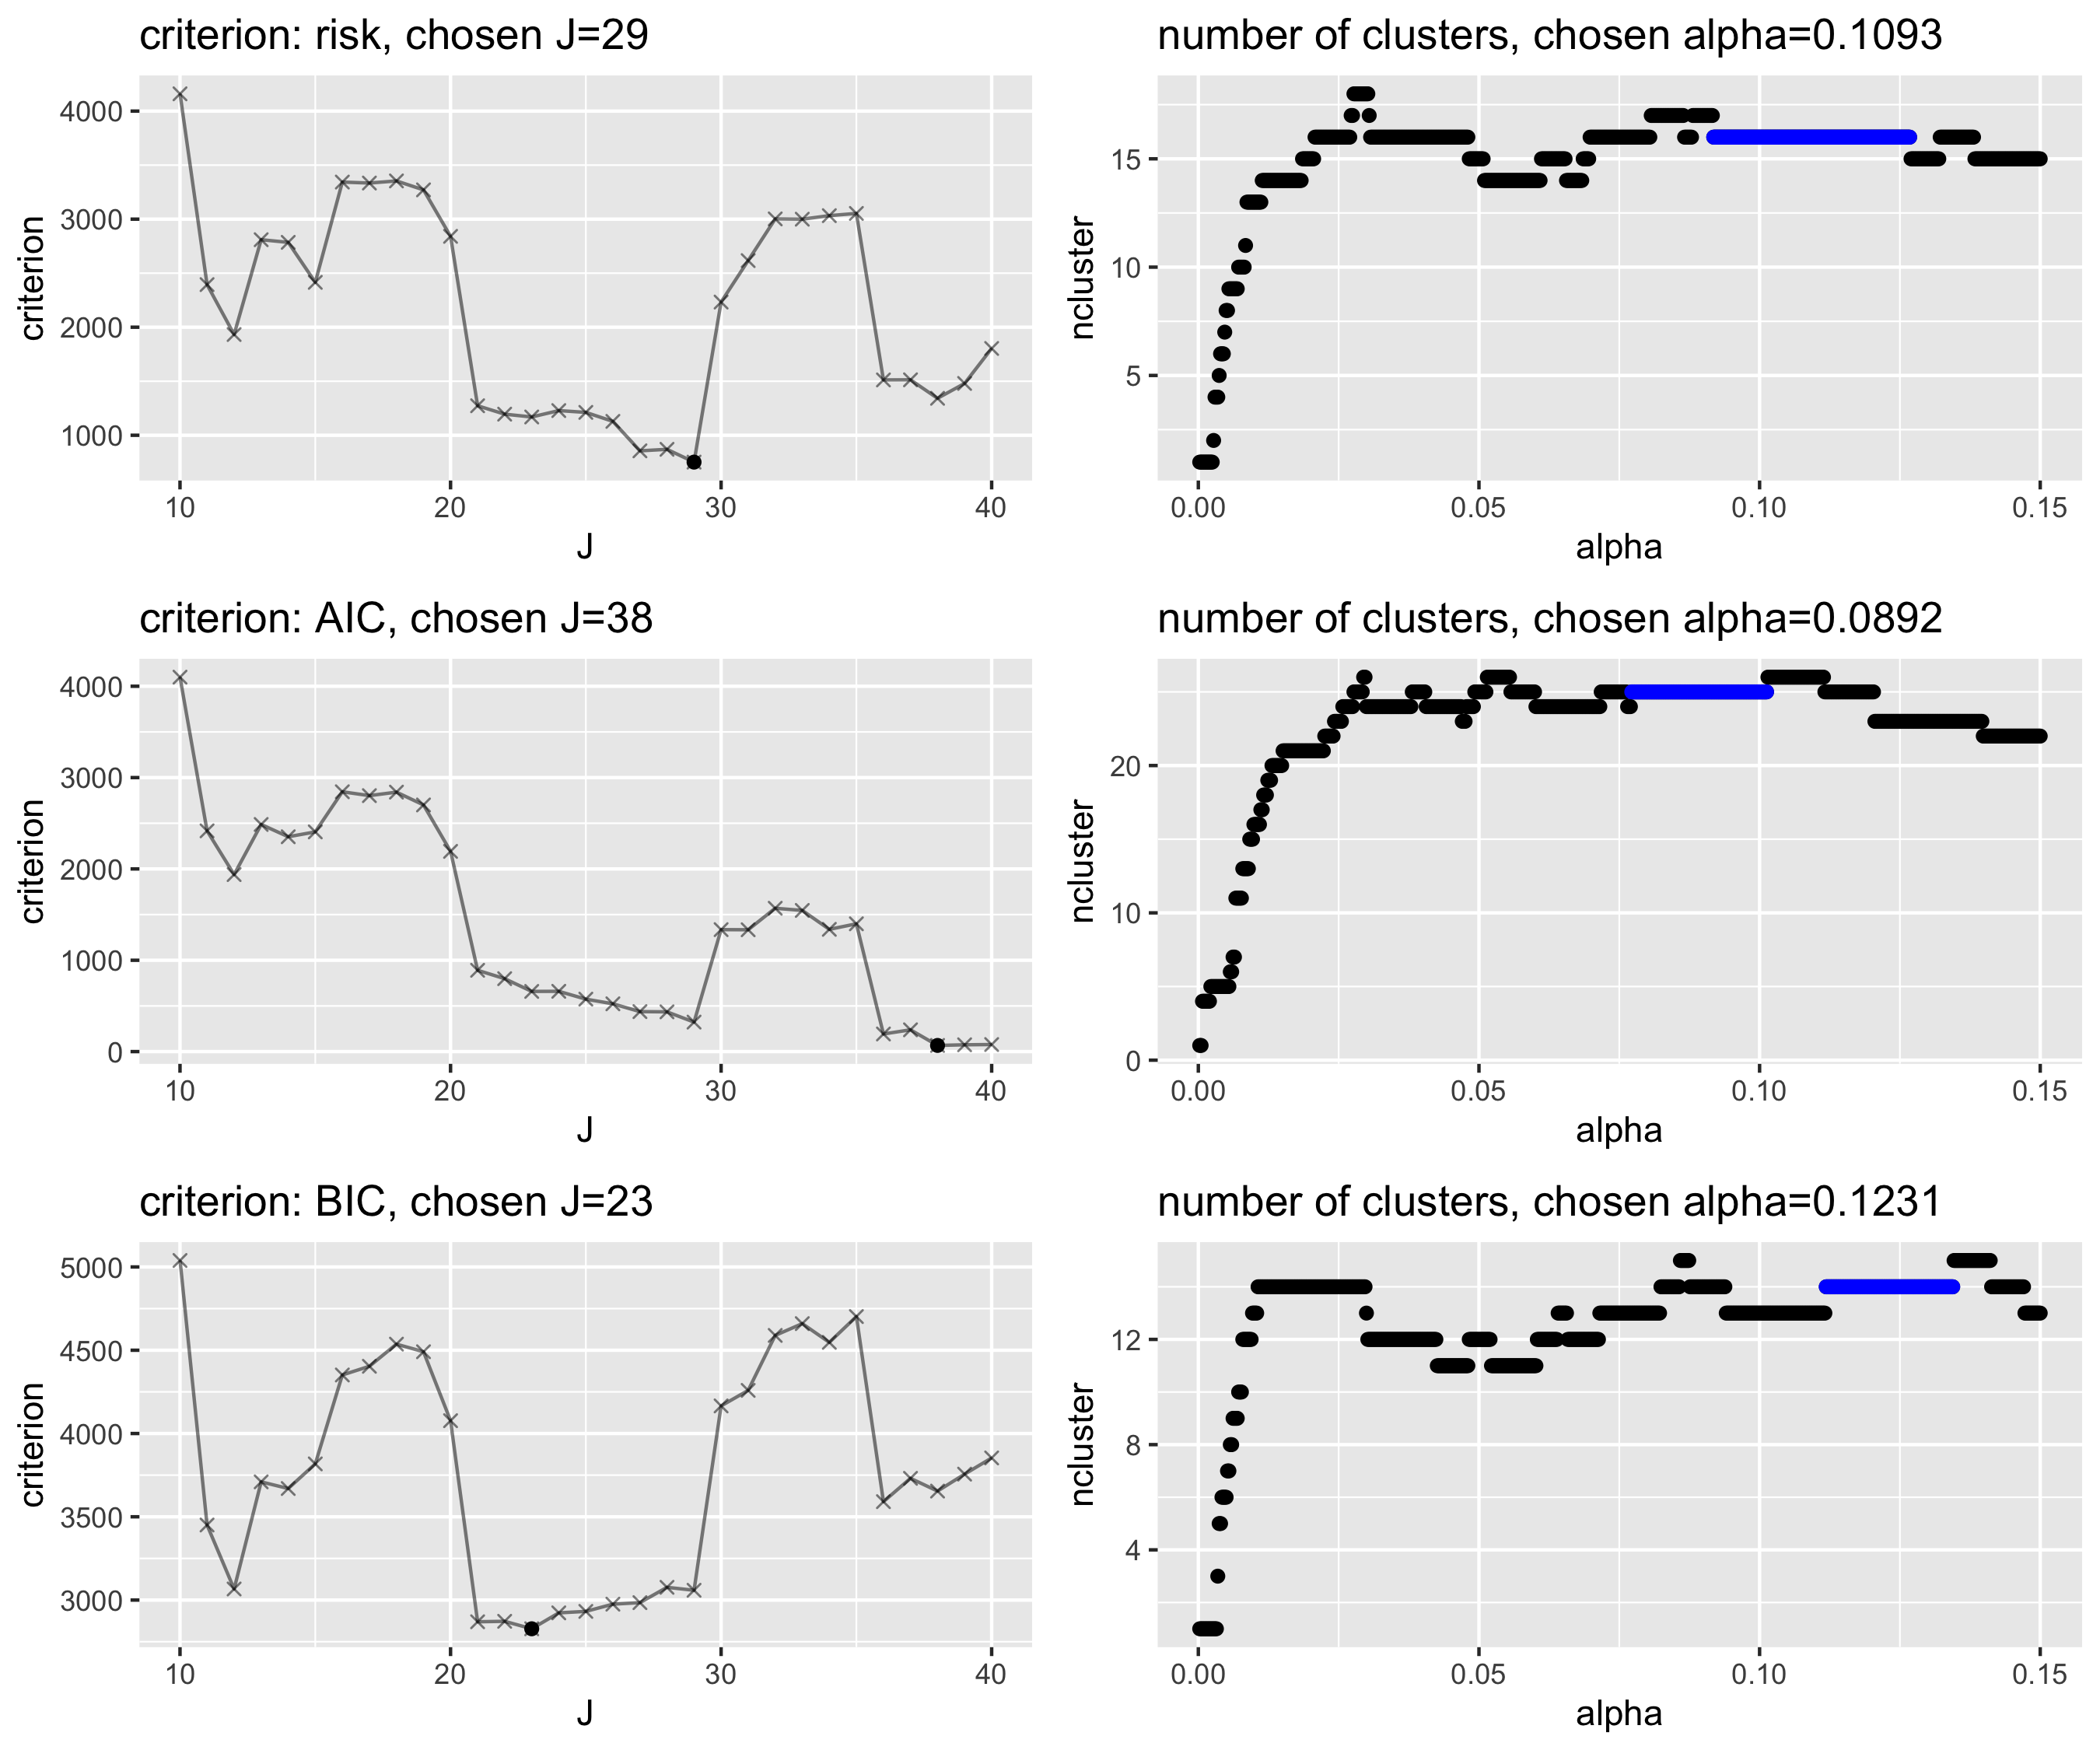
\includegraphics[scale = 0.147]{criterion.png}
     \caption{Hyperparameter selection for \code{ILE} data, generated from the outputs of \code{hyperparam.torus}. Rows correspond to different choices of criteria "risk", "AIC" and "BIC". In each row, the left panel shows the values of criterion over $J$, with the optimal $\hat{J}$ indicated by a thicker dot; the right panel shows the number of clusters over varying $\alpha$, in which the longest streak is highlighted. The optimal $\hat\alpha$ is the midpoint of the longest streak.}
     %The plots for the designated criterion and the number of clusters by varying $J$ and $\alpha$ respectively. Left column panels are for the criterion versus $J$ and the right column panels for the number of clusters versus various level $\alpha$. Top row panels represents the argument \code{option="risk"}, middle panels for \code{option="AIC"}, and the bottom panels for \code{option="BIC"}. {\color{red}Note that dot points in left column panels indicate the optimal $J$, and blue lines in right column panels indicate the longest interval $I$ where the number of clusters does not change by varying the level. The first row of this plot is generated with the code \code{plot(output\_list\$risk)} and the second and third row are also generated in the same manner.}} 
     \label{fig:criterion}
\end{figure}

The number of clusters, given by the conformal prediction set $C_n(\hat\alpha,\hat{J})$, can be seen in the right panels of Figure \ref{fig:criterion}. For example, in the top right panel, with $\hat{J} = 29$ and $\hat\alpha = 0.1093$, the number of clusters is 16 (the vertical position of the blue-colored longest streak). 
For the subsequent analysis, we use the risk criterion, thus choosing $(\hat{J}, \hat\alpha) = (29, 0.1093)$.

\begin{example}
hyperparam.risk.out <- output_list$risk
\end{example}

Finally, the function \code{cluster.assign.torus} is used for cluster membership assignment for each data point in \code{ILE}. In the code below, the function \code{cluster.assign.torus} takes as input \code{hyperparam.risk.out}, an output of \code{hyperparam.torus}, and we have not specified any level. 
Since the object \code{hyperparam.risk.out} contains the chosen level $\hat\alpha$ (in its value \code{alphahat}), the level of the conformal prediction set is, by default, set as \code{hyperparam.risk.out\$alphahat}.

\begin{example}
cluster.out <- cluster.assign.torus(hyperparam.risk.out)
\end{example}

The output \code{cluster.out} contains the membership assignment results as well as the number of clusters, which can be retrieved by \code{cluster.out\$ncluster} or by simply printing the output \code{cluster.out}. 
The assigned cluster memberships can be displayed on the pairwise scatter plots of the four angles. We demonstrate the outlier-disposing membership assignment (the default behavior for S3 method \code{plot}), as well as the membership assignment based on the maximum of log-densities. Figure \ref{fig:cluster_ile} displays the scatter plots generated by the codes:  


\begin{figure}[p]
     \centering
     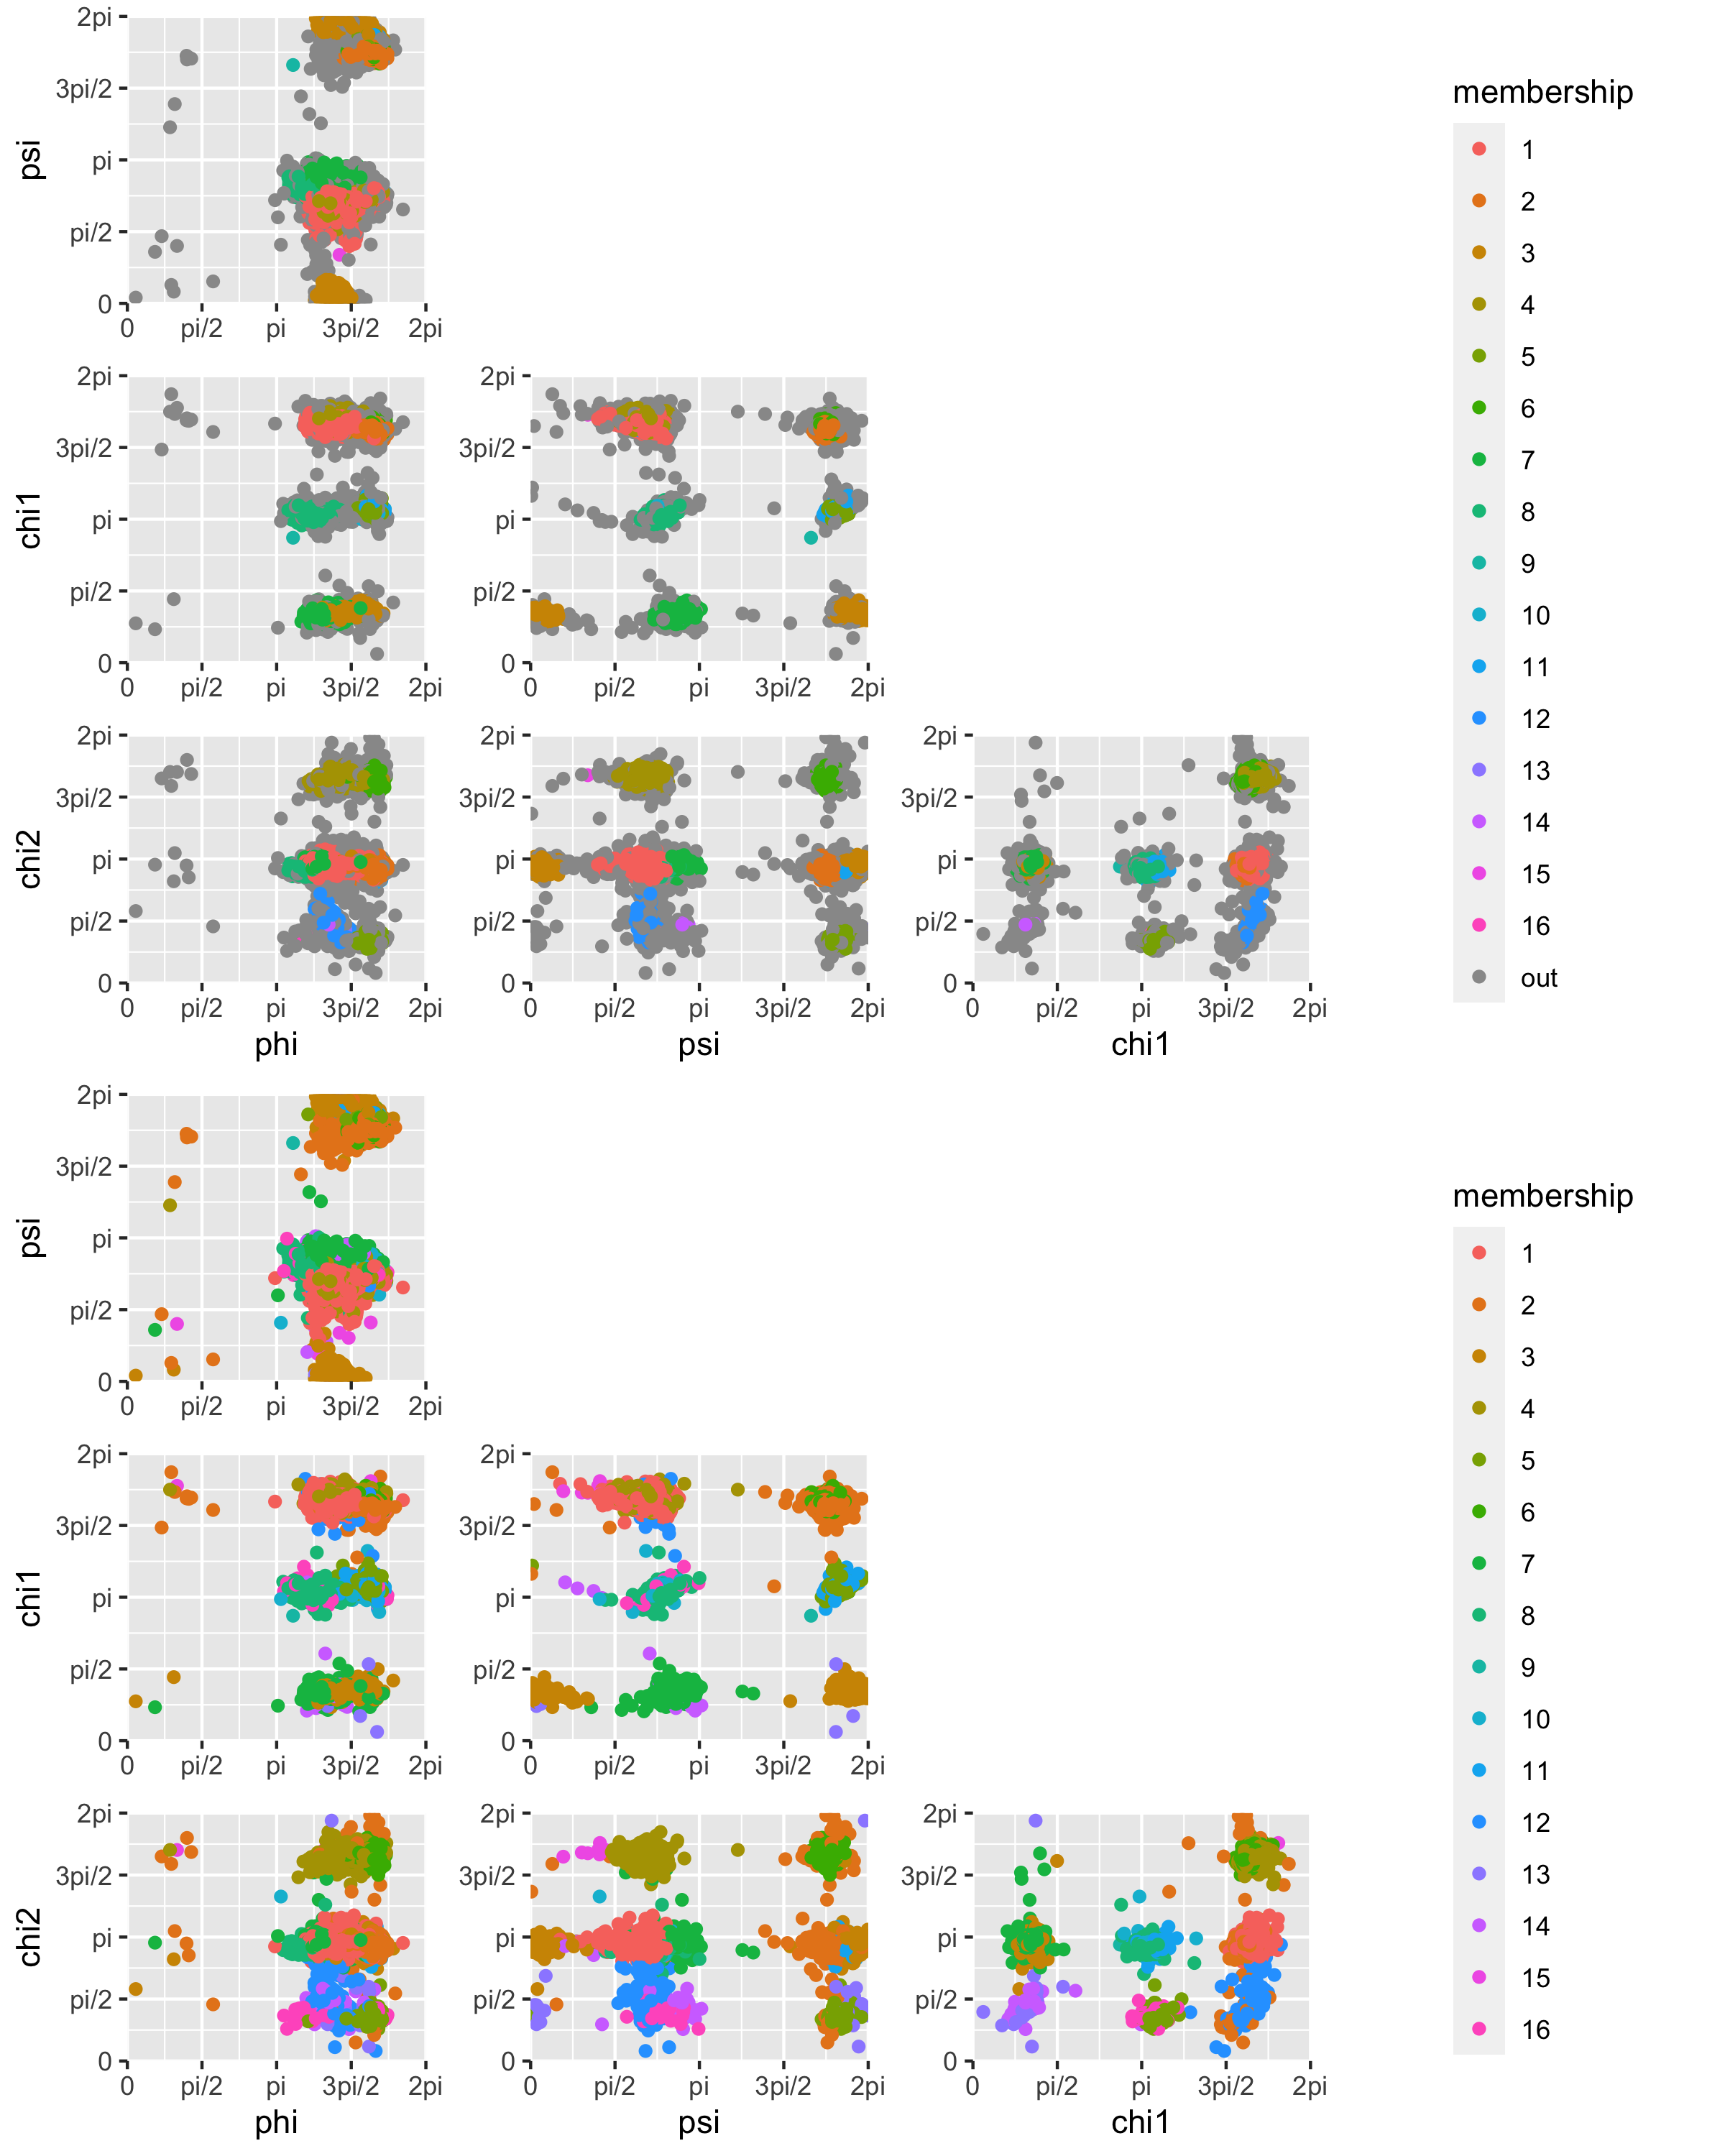
\includegraphics[scale = 0.165]{cluster_ile.png}
     \caption{The pairwise scatter plots of \code{ILE} data with cluster assignments. (Top) \code{assignment = "outlier"}. (Bottom) \code{assignment = "log.density"}.}
     \label{fig:cluster_ile}
\end{figure}


\begin{example}
plot(cluster.out, assignment = "outlier")     # Top panel of Figure 7
plot(cluster.out, assignment = "log.density") # Bottom panel of Figure 7
\end{example}


Note that these cluster assignments are based on the conformal prediction set $C_n(\hat\alpha,\hat{J})$. The information to construct $C_n(\alpha, \hat{J})$ (for any $\alpha \in (0,1)$) is contained in the object \code{hyperparam.risk.out} as value \code{icp.torus}. Since the conformal prediction set is a union of 4-dimensional toroidal ellipsoids, projections of such ellipsoids onto coordinate planes are plotted by the following code, and is shown in Figure \ref{fig:circ_ile}.
 
\begin{figure}[t]
     \centering
     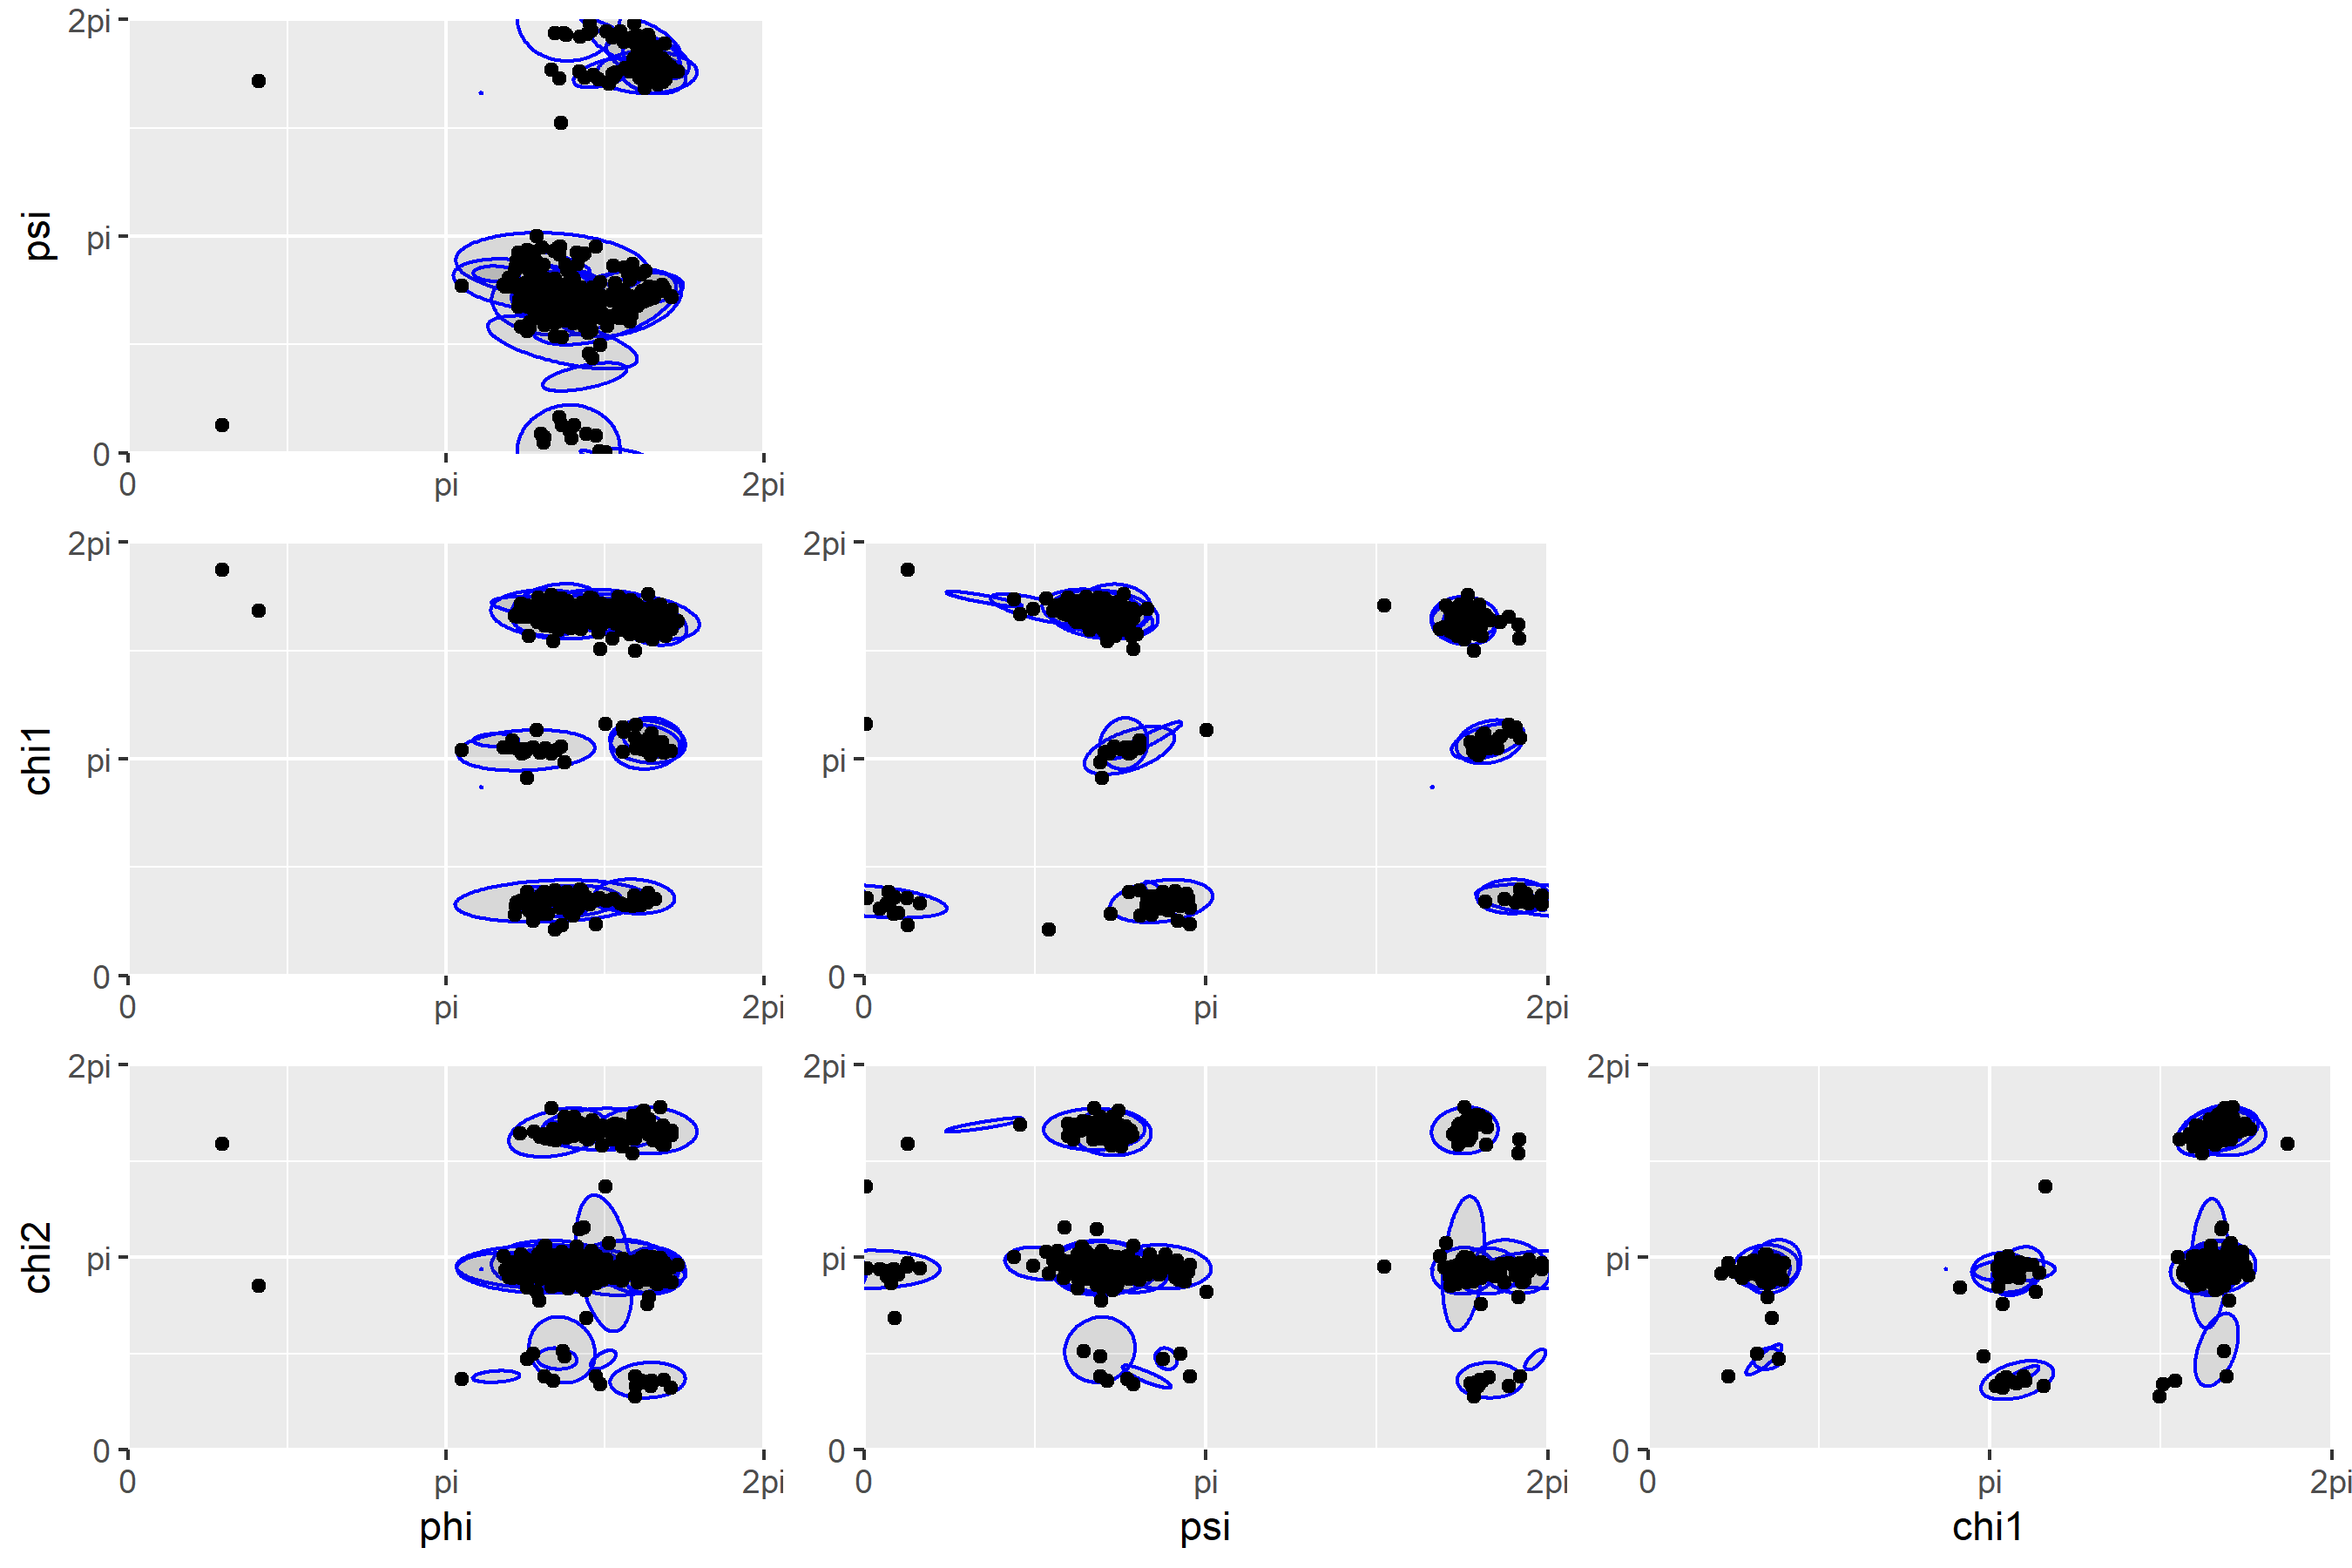
\includegraphics[scale = 0.6]{circ_ile.png} % 0.148
     \caption{The pairwise scatter plots of \code{ILE} data, overlaid with the (projected) ellipsoids that constitute  the conformal prediction set $C_n(\hat\alpha,\hat{J})$.}
     \label{fig:circ_ile}
\end{figure}

\begin{example}
set.seed(2021)
plot(hyperparam.risk.out$icp.torus, 
     data = ILE[sample(1:nrow(ILE),500),], 
     level = hyperparam.risk.out$alphahat) 
\end{example} 

Scatter plots of $n = 8080$ observations are typically too busy, especially when other information (such as the ellipses) is overlaid. In the code example above, we use the argument \code{data = ILE[sample(1:nrow(ILE),500),]}  to plot randomly selected observations. 

%Because the data is on the four-dimensional torus, it seems difficult to evaluate the performance of clustering with the colored scatter plots visually. Nevertheless, considering Figure \ref{fig:circ_ile}, it seems that the performance of clustering is satisfactory.


%In the codes above, 16 clusters are identified and cluster labels are assigned by \code{cluster.assign.torus}. The result is illustrated in Figure \ref{fig:cluster_ile} and Figure \ref{fig:circ_ile}. Figure \ref{fig:cluster_ile} displays the cluster assignment with colors, and Figure \ref{fig:circ_ile} visualizes the projection of the generated conformal prediction set to each coordinate plane. Because the data is on the 4 dimensional torus, it seems difficult to check the performance of clustering with the colored scatter plots visually. Nevertheless, considering Figure \ref{fig:circ_ile}, it seems that the performance of clustering is satisfactory. Note that clustering plot as Figure \ref{fig:cluster_ile} and ellipsoid plot \ref{fig:circ_ile} are generated with the following codes respectively:







%{\color{blue} Since the data are in $\mathbb{T}^4$, it is computationally infeasible to use the criterion \eqref{eq:16} for selecting optimal hyperparameters, because of extremely many grid points.} Rather than using \code{option="elbow"}, the following codes use \code{option="risk"},  \code{"AIC"}, and \code{"BIC"} of \code{hyperparam.torus}. To find the optimal $J$, we vary $J$ from {\color{red}10} to 40 and fit the models with the elliptical $k$-means algorithm. The codes also exhibit the two different ways of cluster assignments.
 

%Figure \ref{fig:criterion} illustrates the hyperparameter selection procedure and choice of $J$ and $\alpha$ for each criterion.
%The choices are $\hat{J}=26$ and $\hat{\alpha}=0.079$ for \code{option="risk"}, $\hat{J}=28$ and $\hat{\alpha}=0.082$ for \code{option="AIC"}, and $\hat{J}=20$ and $\hat{\alpha}=0.076$ for \code{option="BIC"}.
%{\color{red}The codes above also suggest that the number of clusters is 16 for \code{option="risk"}, 25 for \code{option="AIC"}, and 14 for \code{option="BIC"}.} The right column of the figure plots the number of clusters over varying level. Setting \code{option="BIC"} tends to choose a simple model compared to the others.
%Options \code{"risk"} and \code{"AIC"} provide similar {\color{red}reformation of graph}; the lengths of the stable intervals and {jumping behaviors} are similar. This may implies that the estimated models for $J=29$ and $J=38$ share some modes and thus the two models are almost the same.
%{\color{red}We choose $J = 29$ and level $\alpha = 0.1093$ given by \code{option="risk"}, for the clustering.}

%In the codes above, 16 clusters are identified and cluster labels are assigned by \code{cluster.assign.torus}. The result is illustrated in Figure \ref{fig:cluster_ile} and Figure \ref{fig:circ_ile}. Figure \ref{fig:cluster_ile} displays the cluster assignment with colors, and Figure \ref{fig:circ_ile} visualizes the projection of the generated conformal prediction set to each coordinate plane. Because the data is on the 4 dimensional torus, it seems difficult to check the performance of clustering with the colored scatter plots visually. Nevertheless, considering Figure \ref{fig:circ_ile}, it seems that the performance of clustering is satisfactory. {\color{red}Note that clustering plot as Figure \ref{fig:cluster_ile} and ellipsoid plot \ref{fig:circ_ile} are generated with the following codes respectively:
 
%\begin{figure}
%     \centering
%     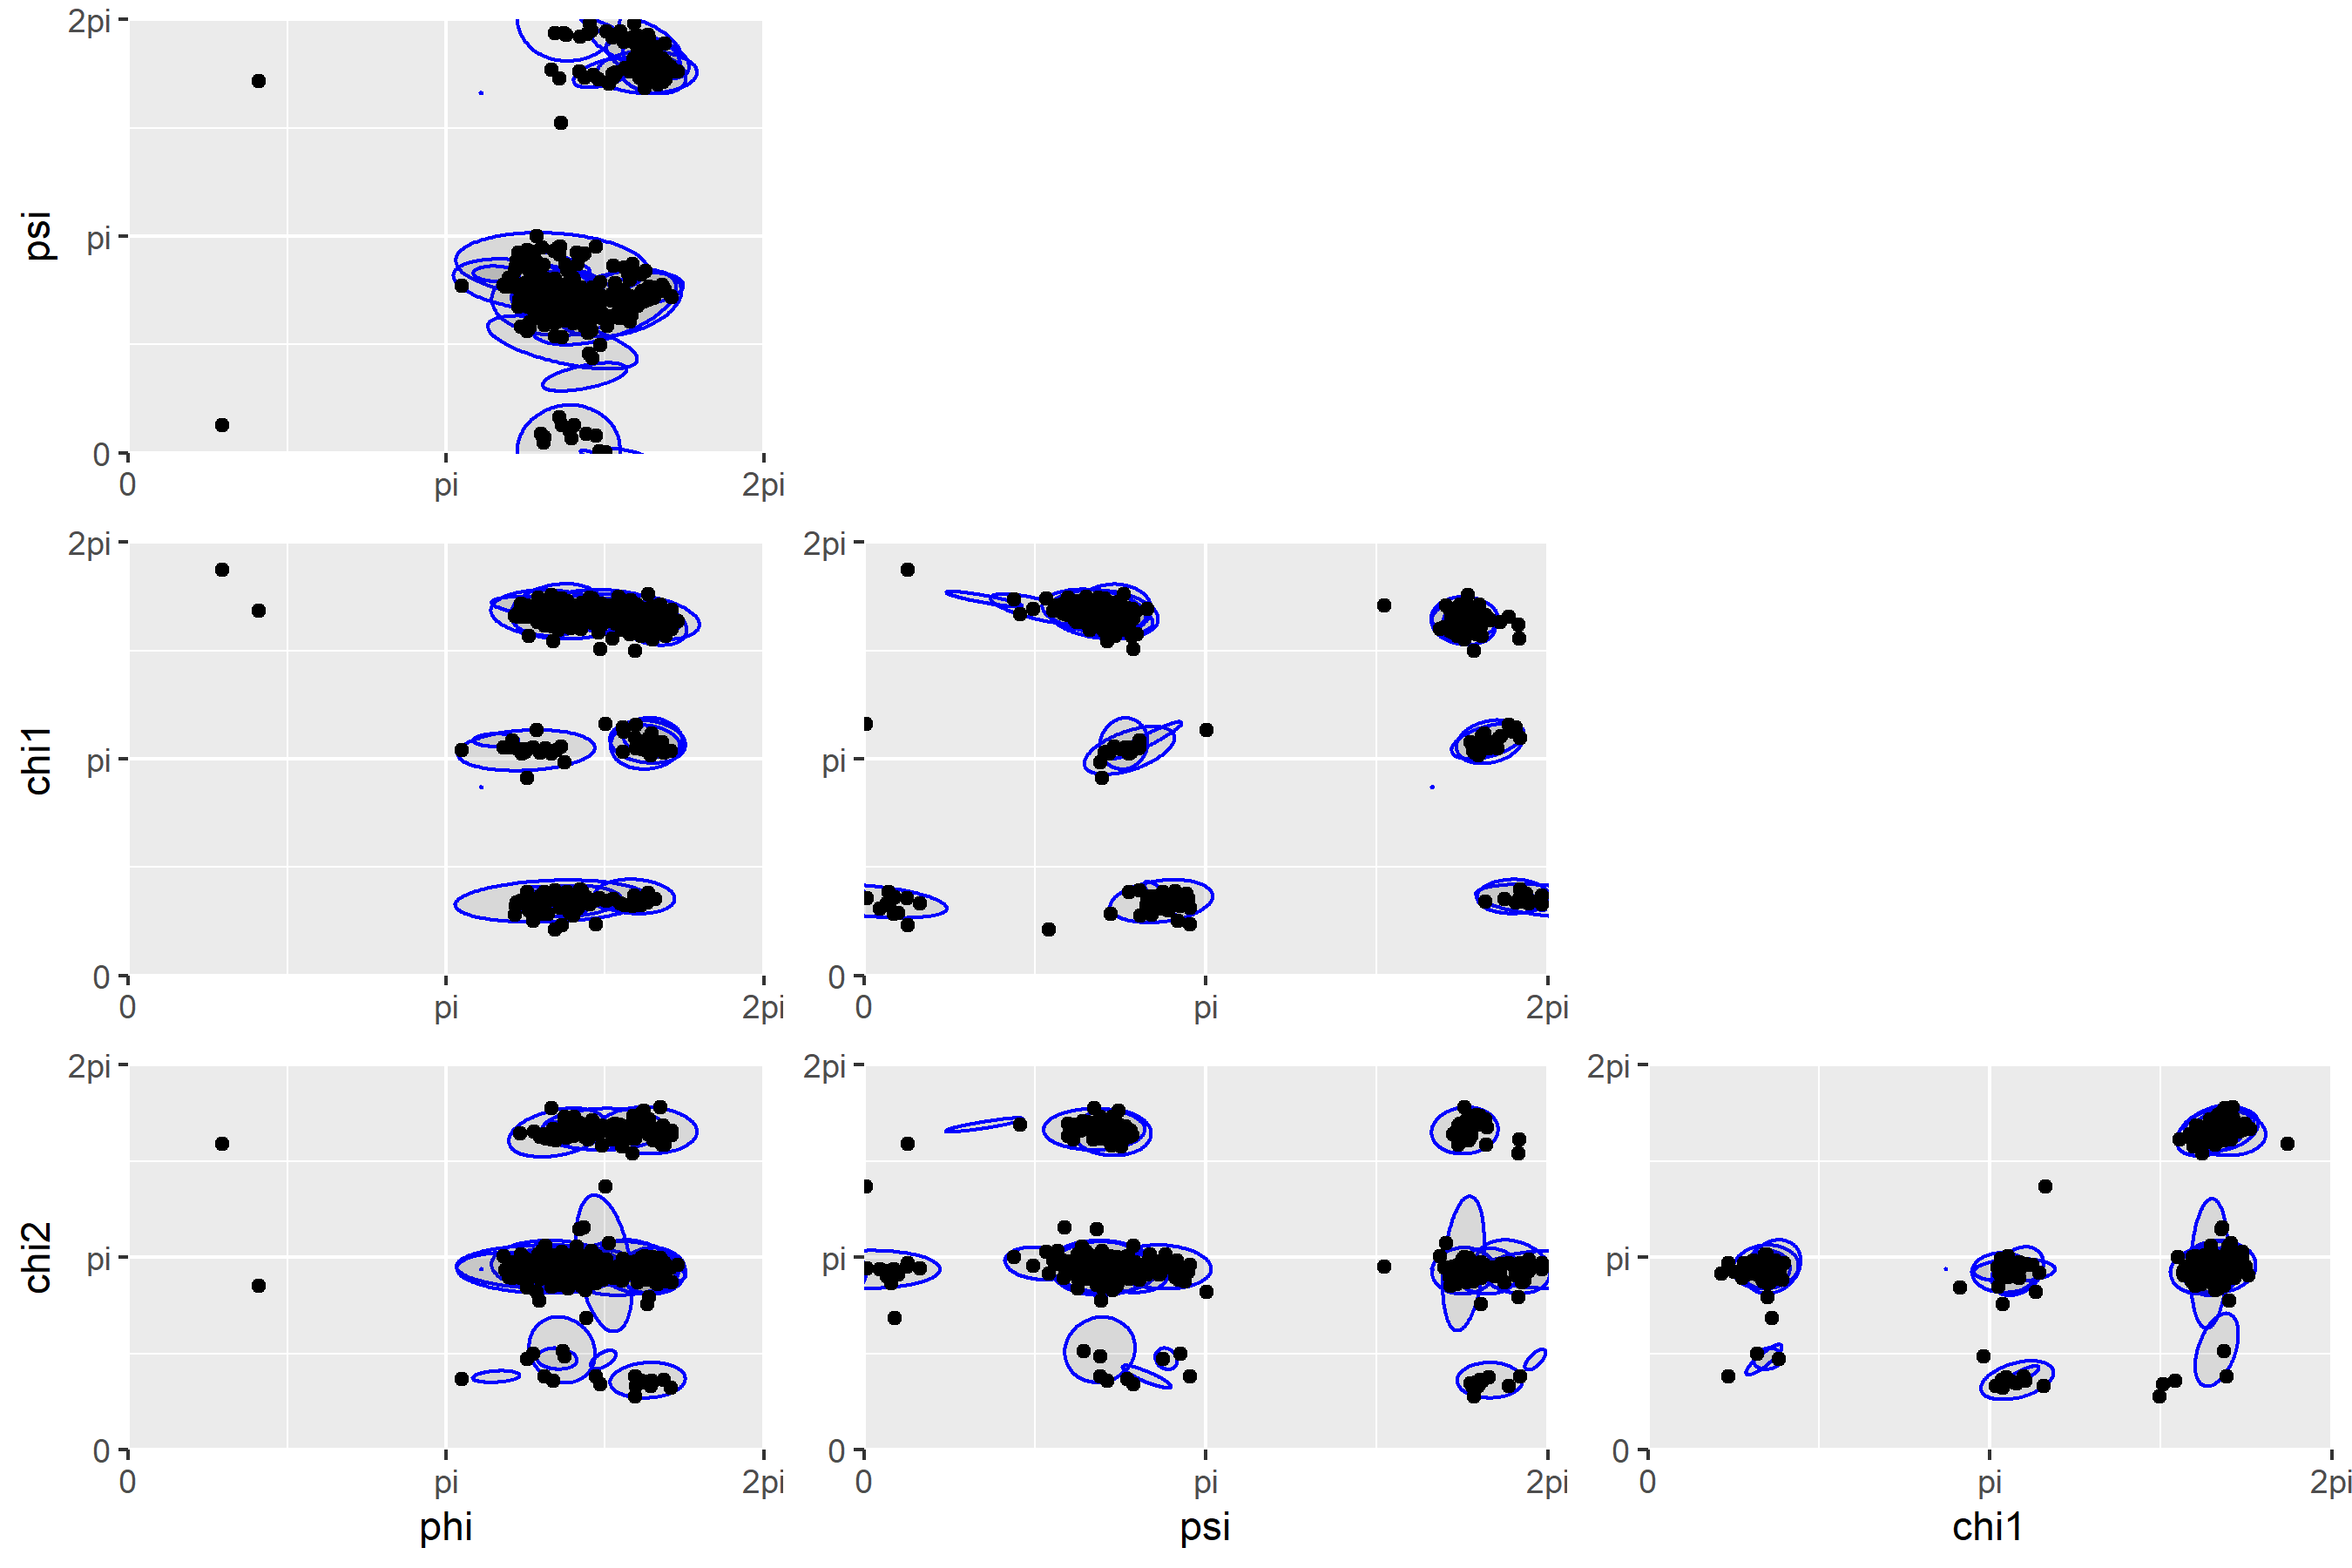
\includegraphics[scale = 0.148]{circ_ile.png}
%     \caption{The pairwise scatter plot for ILE data with conformal preidction set whose conformity score is \eqref{eq:12} under the \code{kmeansfitmethod = "general"} condition in \code{cluster.assign.torus}, with $J = 29$ for level $\alpha = 0.1093$. Each panel shows 2-dimensional projection of the conformal prediction set for the selected two coordinates with the corresponding scatter plot.}
%     \label{fig:circ_ile}
%\end{figure}

\section{All-in-one function: \code{clus.torus}}

The predictive clustering for data on the torus is obtained by sequentially applying functions \code{icp.torus}, \code{hyperparam.torus} and \code{cluster.assign.torus}, as demonstrated for \code{ILE} data in the previous section. The function \code{clus.torus} is a user-friendly all-in-one function, which performs the predictive clustering by sequentially calling the three core functions. 

Using \code{clus.torus} can be as simple as \code{clus.torus(data)}, as shown in the first code example, resulting in Figure~\ref{fig:covid}, in Introduction. In this case, the three functions are called sequentially with default choices for their arguments. On the other hand, users can specify which models and fitting methods are used, whether hyperparameter tuning is required, and, if so, which criterion is used for \code{hyperparam.torus}, and so on. 
%
Key arguments of \code{clus.torus} are summarized in Table~\ref{table:clus.torus}. 
The argument \code{model} only takes \code{"kmeans"} and  \code{"mixture"} as input, which is passed to \code{icp.torus} inside the function. Since the function concerns clustering, conformal prediction sets consisting of ellipsoids \eqref{eq:12} are needed, and such prediction sets are given by both \code{model = "kmeans"} and  \code{"mixture"}. 
Next, the values of the arguments \code{J} and \code{level} determine whether tuning is needed for hyperparameters $J$ and $\alpha$. If both are not specified, i.e., \code{J = NULL} and \code{level = NULL}, then \code{hyperparam.torus} is used to select both parameters, with argument \code{option} (see  Table~\ref{table:clus.torus}). If either \code{J} or \code{level} is specified as a scalar, then the function simply uses the given value for constructing the conformal prediction sets and for clustering. Other arguments available for \code{icp.torus} and \code{hyperparam.torus} can be specified, and the function passes those arguments to corresponding functions, if applicable.

%On the other hand, there are a number of arguments available. Most of these arguments are passed to either \code{icp.torus} or \code{hyperparam.torus}. We summarize 


\renewcommand{\arraystretch}{1.1}
\begin{table}[hbt!]
\small
\begin{tabularx}{\textwidth}{lX}
\toprule
Arguments       &  Descriptions \\\hline
\code{data}     &  $n \times d$ matrix of toroidal data on $[0, 2\pi)^d$ or $[-\pi, \pi)^d$ \\ \hline
\code{model}   &  
A string. One of \code{"kmeans"} and  \code{"mixture"} which
  determines the model or estimation methods. If \code{"mixture"}, the model is the von Mises mixture, fitted
  with an EM algorithm.  If \code{"kmeans"}, the model is also the von
   Mises mixture, fitted by the elliptical k-means algorithm. If the
   dimension of data space is greater than 2, only \code{"kmeans"} is supported.
   Default is \code{model = "kmeans"}.\\ 
\hline
\code{J}       &  A scalar or numeric vector. If \code{J} is scalar, the number of components $J$ is set as \code{J}. If \code{J} is a vector,
       then \code{hyperparam.torus} or \code{hyperparam.J} is used to select $\hat{J}$. Default is 
       \code{J = NULL}, in which case \code{J = 4:30} is used. \\ \hline
\code{level}   & A scalar in $[0,1]$. The level of the conformal prediction set
  used for clustering. Default is \code{level = NULL}, in which case \code{hyperparam.alpha} is
  used to choose optimal \code{level} $\hat\alpha$.  \\ \hline
\code{option}  &     A string. One of \code{"elbow"}, \code{"risk"}, \code{"AIC"}, or \code{"BIC"}, determining the criterion used for \code{hyperparam.torus} andr \code{hyperparam.J}. Default is \code{option = "elbow"} if $d = 2$, and \code{option = "risk"} if $d > 2$.\\ \hline
\bottomrule
\end{tabularx}
\caption{Key arguments and descriptions of the function \code{clus.torus}}
\label{table:clus.torus}
\end{table}


%As a summary of our implementation, we introduce the function \code{clus.torus}, which was demonstrated for Figure 1 in Introduction. The function \code{clus.torus} uses arguments \code{model}, \code{kmeansfitmethod}, \code{mixturefitmethod}, and \code{J} of the function \code{icp.torus}. With these arguments, \code{clus.torus} evaluates model parameters and conformity scores. Note that the argument \code{model} only takes one of \code{model = "kmeans"} or \code{model = "mixture"}. That is, \code{clus.torus} does not support the model based on kernel density estimation. Next, with arguments \code{level} and \code{option}, as \code{hyperparam.torus}, \code{clus.torus} selects $\hat{J}$ and level $\hat{\alpha}$ under criterion \code{option}. Finally, with  $\hat{J}$ and $\hat{\alpha}$, as \code{cluster.assign.torus}, it generates clusters by varying clustering rules. In other words, the function \code{clus.torus} is a combination of \code{icp.torus}, \code{hyperparam.torus}, and \code{cluster.assign.torus}, and returns \code{clus.torus} object which consists of the outputs of these 3 functions.

The output of the function is a list of three objects, with S3 class \code{clus.torus}. The three objects in the output are 
\begin{enumerate}
    \item a \code{cluster.obj} object, containing the results of cluster membership assignments,
    \item an \code{icp.torus} object, corresponding to the model with $\hat{J}$ (or the specified \code{J}), and
    \item if applicable, a \code{hyperparam.torus}, \code{hyperparam.J} or \code{hyperparam.alpha} object.
\end{enumerate}
Each of these objects can be plotted via \code{plot}, defined for S3 class \code{clus.torus}. 
For example, recall that \code{ex} is a \code{clus.torus} object we created in Introduction. By setting the argument \code{panel} of the method \code{plot} as \code{panel = 1}, the \code{cluster.obj} object is plotted. 

\begin{example}
plot(ex, panel = 1) # equivalent to plot(ex)
\end{example}

The result is shown in Figure \ref{fig:covid} (top left). If the data dimension is $p > 2$, then figures similar to  Figure \ref{fig:cluster_ile} will be created. If \code{panel = 2}, the \code{icp.torus} object is plotted, similar to Figures \ref{fig:ellipse} and \ref{fig:circ_ile}.  Finally, if \code{panel = 3},  the graphics relevant to hyperparameter selection are created, similar to Figure \ref{fig:criterion}.

 
% If \code{panel = 1}, then it plots its \code{cluster.obj} output as Figure \ref{fig:cluster_ile} and upper-left panel of Figure \ref{fig:covid}. If \code{panel = 2}, it plots \code{icp.torus} output as Figure \ref{fig:ellipse} and \ref{fig:circ_ile}. If \code{panel = 3}, it plots \code{hyperparam.torus} output as Figure \ref{fig:criterion}. Hence, we can get almost all outputs we have shown with this function.




%On the other hand, \code{clus.torus} has a S3 plot method, with argument \code{panel}. This argument takes a value one of 1,2 and 3. If \code{panel = 1}, then it plots its \code{cluster.obj} output as Figure \ref{fig:cluster_ile} and upper-left panel of Figure \ref{fig:covid}. If \code{panel = 2}, it plots \code{icp.torus} output as Figure \ref{fig:ellipse} and \ref{fig:circ_ile}. If \code{panel = 3}, it plots \code{hyperparam.torus} output as Figure \ref{fig:criterion}. Hence, we can get almost all outputs we have shown with this function.

\section{Other methods of clustering on the torus}

\citet{Gao:2018} and \citet{Jung:2021} used the \dfn{extrinsic $k$-means}, which uses Euclidean embedding and enjoys fast computation of the vanilla $k$-means algorithm. That is, consider the mapping $f:\mathbb{T}^p\rightarrow\mathbb{R}^{2p}$
as
$$
f\left(\phi_1,\cdots,\phi_p\right) = \left(\cos{\phi_1},\cdots,\cos{\phi_p},\sin{\phi_1},\cdots,\sin{\phi_p}\right)
$$
which is the simple Euclidean embedding and is injective. Since $\mathbb{R}^{2p}$ is a Euclidean space, the $k$-means clustering for vector-valued data can be used. The function \code{kmeans.torus} implements the extrinsic $k$-means clustering. In the simple code example below, the number of cluster is set to $k = 3$,  and the result shows the membership assignment by the extrinsic $k$-means algorithm. 
\begin{example}
set.seed(2021)
exkmeans <- kmeans.torus(SARS_CoV_2, centers = 3, nstart = 30)
head(exkmeans$membership)

  27.B.ALA   28.B.TYR   29.B.THR   30.B.ASN   31.B.SER   32.B.PHE
         1          1          1          1          2          3
\end{example}

Distance-based clustering methods, such as hierarchical clustering, only requires a pairwise distances of the data points. The function \code{ang.pdist} generates the distance matrix for the input data in which the angular distance between the two points on $\mathbb{T}^p$ is measured. Combined with \code{hclust}, the pairwise angular distances are used to provide a hierarchical clustering using, e.g., the complete linkage, as done in the following example.
%An example showing a hierarchical clustering is given below:
\begin{example}
distmat <- ang.pdist(SARS_CoV_2)
hc <- hclust(distmat, method = "complete")
hc.result <- cutree(hc, k = 3)
head(hc.result)

[1] 1 1 1 1 2 3
\end{example}

Figure \ref{fig:others} shows the results for the two clustering algorithms, discussed above. The left panel shows that the Euclidean embedding reflects the rotational nature of angular data. The right panel shows that the distance-based clustering methods is well-applied with \code{ang.pdist}.  Note that both the extrinsic $k$-means and the hierarchical clustering results are invariant to different representations of angles. That is, the cluster assignments do not change if $\mathbf{X}_n$ is replaced by $\mathbf{X}_n - \pi$. However, these methods are inadequate when true clusters are irregularly shaped and when there are outliers \citep{Jung:2021}. In addition, the number of clusters needs to be predetermined for both methods. In contrast, these weaknesses are mostly resolved by using the predictive clustering.



\begin{figure}[hbt!]
     \centering
     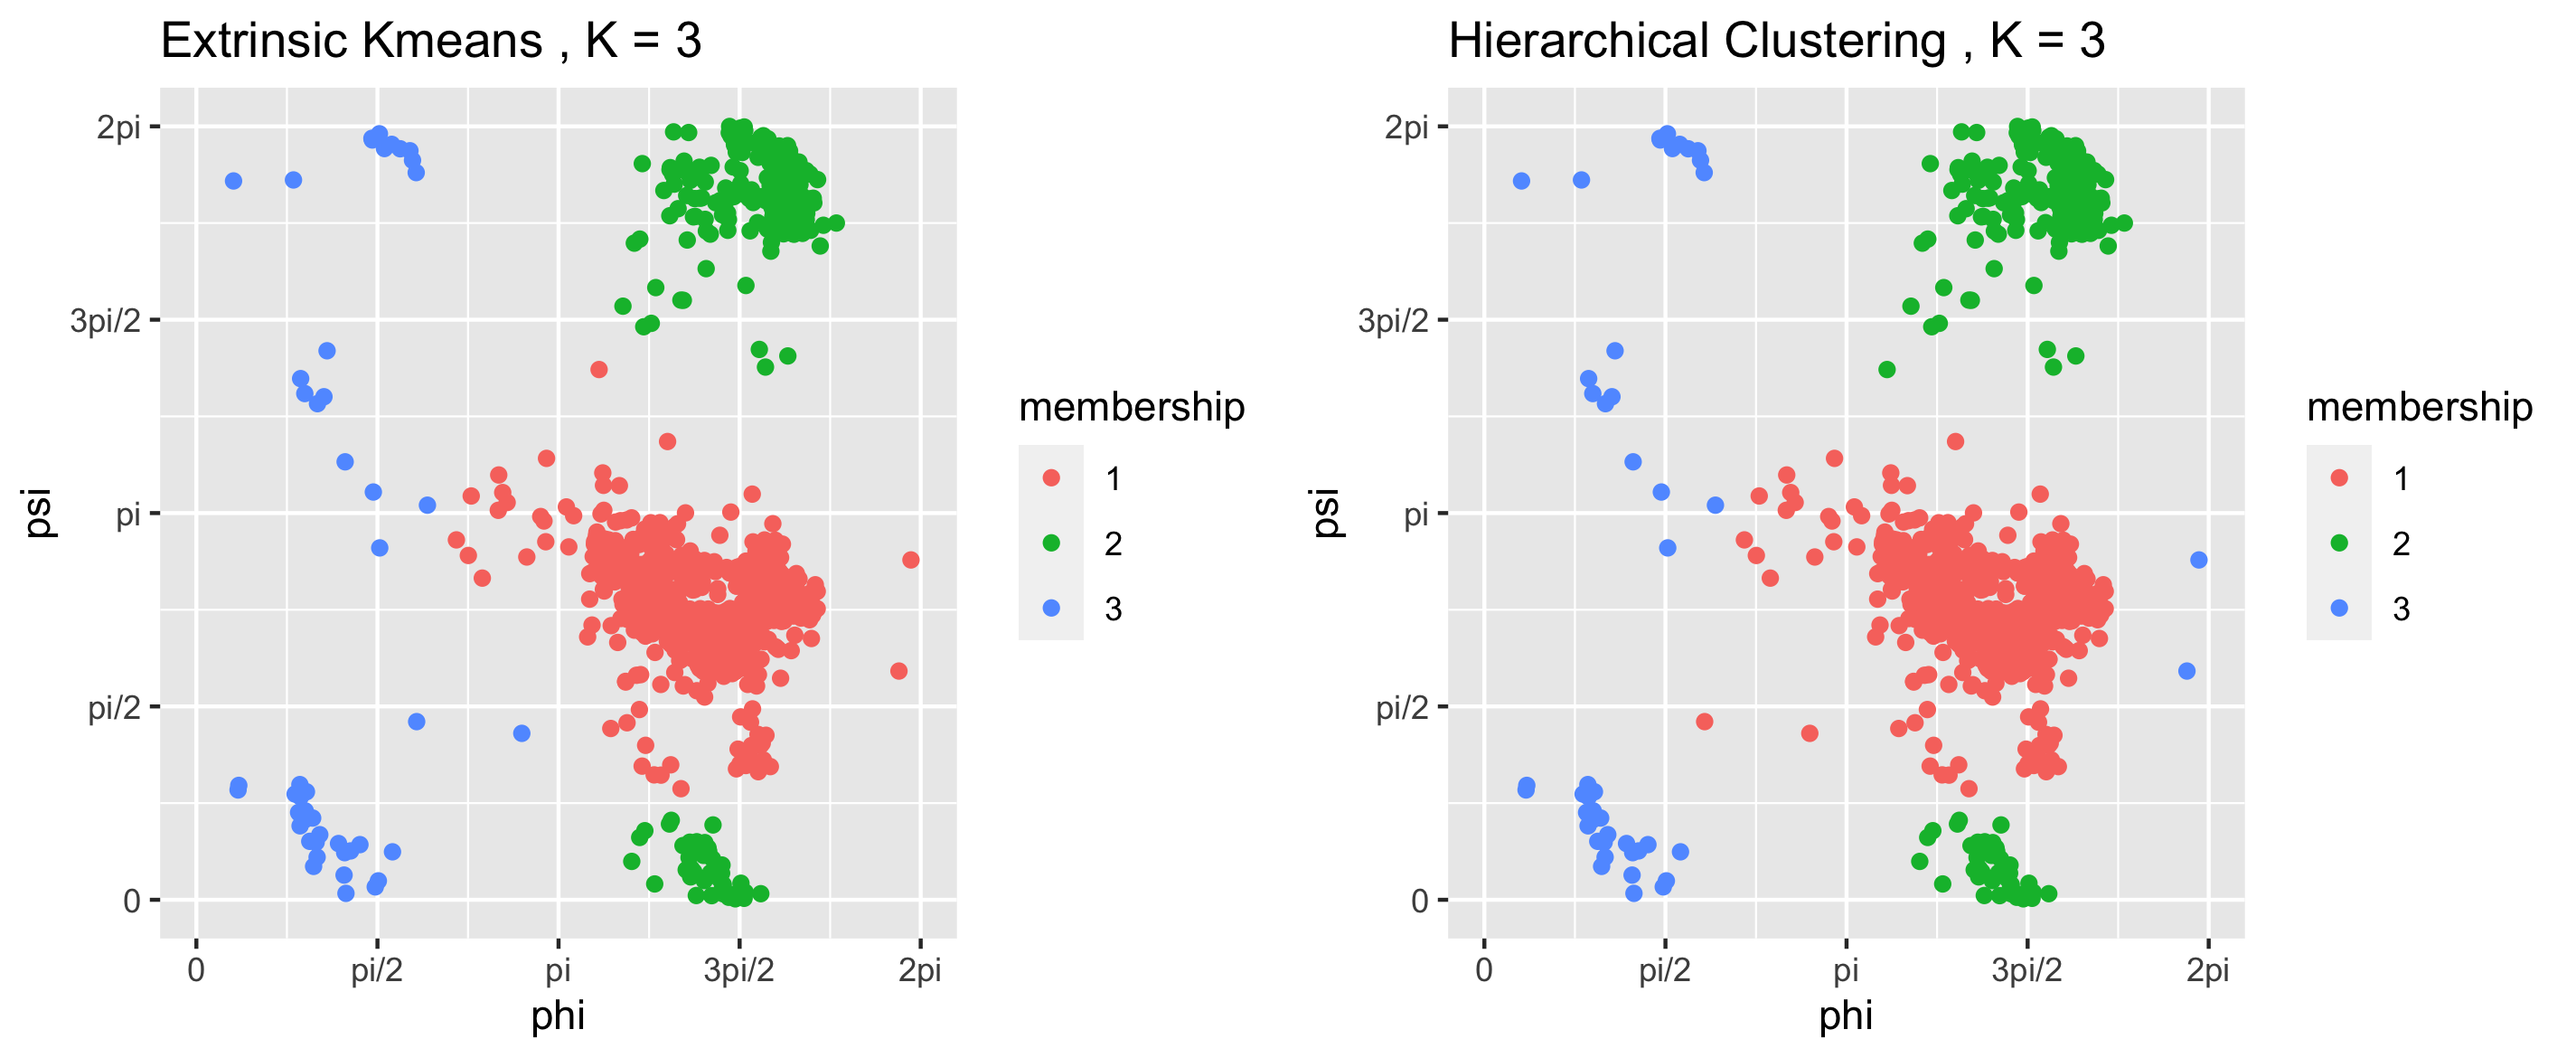
\includegraphics[scale = 0.135]{others.png}
     \caption{The clustering results for SARS-CoV-2 by using extrinsic $k$-means and hierarchical clustering under the 3 clusters assumption. The left panel shows the result for extrinsic $k$-means, and the right panel shows the result for hierarchical clustering.}
     \label{fig:others}
\end{figure}

%{\color{red} On the other hand, since the cyclic nature of angles is not reflected in normal distributions, Gaussian mixture models, which may be fitted by \pkg{mclust} and \pkg{mixtools} (DO WE NEED CITATIONS?), are generally not appropriate for multivariate angles. Clustering results obtained by blindly fitting Gaussian mixtures are shown in Fig.~\ref{fig:GaussMixWrong}, in which an obvious cluster near the horizontal boundary $\psi = 0 = 2\pi$ is split into two or more clusters.
%}
%\begin{figure}[hbt!]
%     \centering
%     \includegraphics[scale = 0.5]{GaussMixWrong.png}
%     \caption{The clustering results for SARS-CoV-2 by using \code{mclust::Mclust} (left), in which the number of components is chosen by BIC, and \code{mixtools::mvnormalmixEM} (right), in which the number of components is specified as three. [REVISE THE FIGURE]}
%     \label{fig:GaussMixWrong}
%\end{figure}

\section{Summary and discussion}
{In this paper, we introduced the package \pkg{ClusTorus} which contains various tools and routines for multivariate angular data, including kernel density estimates and mixture model estimates. \pkg{ClusTorus} performs clustering based on conformal prediction sets. We demonstrated our implementation with data on $\mathbb{T}^4$. The clustering by \pkg{ClusTorus} can result in cluster assignment either with or without an outlier class. A reviewer pointed out that the package \CRANpkg{MoEClust} \citep{murphy2020gaussian, murphy2021package} can also dispose some points as outliers. However, \pkg{MoEClust} only works on Euclidean space, not on $\mathbb{T}^p$.

There are some possible future developments for \pkg{ClusTorus}. First, EM algorithms for von Mises mixture models on high dimensional tori (e.g., $\mathbb{T}^4$) can be implemented assuming independence of angles in each component. Using closed-form approximations of maximum likelihood estimators for univariate von Mises-Fisher distributions \citep{Banerjee2005, Hornik2014}, fitting mixtures of product components can be done efficiently \citep{grim2017approximation}.
Another direction is obtained by viewing clustering based on \eqref{eq:14} by varying $\alpha$ as surveying birth and death of connected components. This can be dealt with a persistence diagram, a concept of topological data analysis. Hence, instead of using Algorithm \ref{hyperparam.alpha}, one may choose desirable $\alpha$ using persistence diagram. 
%This can also be a future development as a new option for \code{hyperparam.alpha}.

}

\section{Appendix}

\subsection{Elliptical $k$-means algorithm}

In this appendix, we outline the elliptical $k$-means algorithm for the data on the torus, implemented in the function \code{ellip.kmeans.torus}. The algorithm is used to estimate the parameters of the mixture model \eqref{eq:8}, approximated as in \eqref{eq:11}. Note that the EM algorithm can be used for parameter estimation for mixture models in low dimensions. The EM algorithms of \citet{Jung:2021} is implemented in the function \code{EMsinvMmix}, but works for $p=2$ only. For $p>3$, EM algorithms suffer from high computational costs \citep{Mardia:2012}. To circumvent this problem, we estimate the parameters by modifying the generalized Lloyd's algorithm \citep{Shin:2019}, also known as the elliptical $k$-means algorithm \citep{Sung:1998, Bishop}. For vector-valued data, \citet{Shin:2019} showed that the elliptical $k$-means algorithm estimates the parameters sufficiently well for the max-mixture density case as \eqref{eq:10}.

Suppose $y_1,\cdots,y_n\in\mathbb{T}^p$ are an independent and identically distributed sample. Using the approximated density \eqref{eq:11}, the approximated likelihood, $L^\prime$, is
\begin{align}
L^\prime\left(\mu, \Sigma\right) = \left(2\pi\right)^{-np/2}\left|\Sigma\right|^{-n/2}\exp\left[-\frac{n}{2}tr\left( S\Sigma^{-1}\right)\right]
\end{align}
where $S=\frac{1}{n}\sum_{i=1}^n \left(y_i\ominus\mu\right)\left(y_i\ominus\mu\right)^T$. Thus, if $\mu$ is known, $\hat{\Sigma} = S$ maximizes $L^\prime$. Following \citet{Mardia:2012}, the mean $\mu$ is estimated as follows. Let $\bar{U}_j = \sum_{i=1}^n \cos\left(y_{ij}\right)/n$ and $\bar{V}_j = \sum_{i=1}^n \sin\left(y_{ij}\right)/n$ for $j=1,\cdots,p$. Then, $\hat{\mu} = \left(\hat{\mu}_1,\cdots,\hat{\mu}_p\right)^T$,
\begin{align}\label{eq:19}
\hat{\mu}_j = \arctan{\frac{\bar{V}_j}{\bar{U_j}}},\quad j=1,\cdots,p
\end{align}
which is the maximum likelihood estimator of mean direction of von Mises-Fisher distribution \citep{Mardia}.

With these approximated maximum likelihood estimators, the elliptical $k$-means algorithm, described in Algorithm \ref{GLA}, maximizes the likelihood corresponding to the max-mixture model \eqref{eq:10}. The algorithm is implemented in the function \code{ellip.kmeans.torus}. 

\begin{algorithm}[hbt!]
\caption{Elliptical $k$-means algorithm for the torus}\label{GLA}
\begin{algorithmic}[1]
\Procedure{Elliptical k-means}{$\{X_1,\cdots,X_n\}, J$}
  \State Initialize $\pi_j, \theta_j = \left(\mu_j,\Sigma_j\right)$, $j=1,\cdots,J$
  \State set \begin{align*}    w_{i,j}&=
\begin{cases}
1, & \mbox{if }j=\arg\max_l\left[-\left(X_i\ominus \mu_l\right)^T\Sigma_l^{-1}\left(X_i\ominus \mu_l\right)-\log\left|\Sigma_l\right|+2\log\pi_l\right] \\
0, & \mbox{otherwise}
\end{cases}\\I_j &= \left\{i\in\left\{1,\cdots,n\right\}|w_{i,j}=1\right\}\end{align*}
  \State Update $\mu_j$ as \eqref{eq:19} with $\left\{X_i\right\}_{i\in I_j}$ for $j=1,\cdots, J$
  \State Update $\Sigma_j=\frac{1}{\sum_{i=1}^nw_{i,j}}\sum_{i=1}^nw_{i,j}\left(X_i\ominus \mu_j\right)\left(X_i\ominus \mu_j\right)^T$ for $j=1,\cdots, J$
  \State Update $\pi_j = \frac{1}{n}\sum_{i=1}^nw_{i,j}$ for $j=1,\cdots, J$
  \State Repeat step 3-6 until converge
\EndProcedure
\end{algorithmic}
\end{algorithm}

Note that the initial values require an initial clustering. For this, we use other clustering algorithms such as the extrinsic $k$-means or the hierarchical clustering algorithms, and can be specified by argument \code{init} of \code{ellip.kmeans.torus} and \code{icp.torus}. One may specify arguments for either \code{hlcust} or \code{kmeans} in \code{icp.torus}. For example, one may specify the choice of initial values as follows.

\begin{example}
icp.torus(data = SARS_CoV_2, J = 4, init = "kmeans", nstart = 30) 
icp.torus(data = SARS_CoV_2, J = 4, init = "hierarchical", method = "complete")
\end{example}

By default, the hierarchical clustering with complete linkage is used. 
Data analysis in this article using \code{icp.torus} or \code{clus.torus} was performed with the default initialization.


\subsection{Constraints for mixture models}

The protein structure data we aim to analyze typically consist of hundreds of angles (observations). Fitting the mixture with a large number of components may give inefficient estimators. Thus, we have implemented options for reducing the number of model parameters, by constraining the shape of the ellipsoids, or the covariance matrices. Applying the constraints lead much faster convergence for estimating parameters \citep{grim2017approximation}. We list three types of constraints for covariance matrices $\Sigma_j$.
These constraints are specified by setting the arguments \code{mixturefitmethod} and \code{kmeansfitmethod} (for \code{icp.torus}) and \code{type} (for \code{EMsinvMmix} and \code{ellip.kmeans.torus}). We explain in terms of the arguments for the function \code{icp.torus}.

%the options to determine the shape of the ellipsoids.
\begin{itemize}
    \item $\Sigma_j=\sigma^2_jI_p$ for some $\sigma^2_j>0$ for all $j$, and the prediction set will be the union of spheres. \code{mixturefitmethod = "circular"} and \code{kmeansfitmethod = "heterogeneous-circular"} represents this constraint. Furthermore, if $\sigma^2_1 = \cdots = \sigma^2_J$ and $\pi_j = 1/J$ for all $j$, then all the spheres have the same radii and this constraint can be designated with \code{kmeansfitmethod = "homogeneous-circular"}.
    \item $\Sigma_j = diag\left(\sigma^2_{jk}\right)_{k=1,\cdots,p}$ for $\sigma^2_{jk}>0$, and the fitted ellipsoids $\hat{E}_j$ $(j=1,\cdots,J)$ are the axis-aligned ellipsoids. \code{mixturefitmethod = "axis-aligned"} represents this constraint.
    \item No constraint for $\Sigma_j$, and $\hat{E}_j$ $(j=1,\cdots,J)$ are any ellipsoids. This option can be designated by \code{mixturefitmethod = "general"} and \code{kmeansfitmethod = "general"}. %(See Table \ref{table:icp.torus.score} for the difference between \code{kmeansfitmethod = "ellipsoids"} and \code{kmeansfitmethod = "general"}.)
    %As a special case, \code{kmeansfitmethod = "ellipsoids"} is used for a one-step update
\end{itemize}

The default values for \code{icp.torus} are \code{kmeansfitmethod = "general"} and \code{mixturefitmethod = "axis-aligned"}.


%\subsection{Additional condition for the elliptical k-means algorithm }
%While proceeding the algorithm \ref{GLA}, there may occur the singular matrix problem. Suppose $card\left(I_j\right)\le p$, where $I_j$ is the index set defined in the procedures of algorithm \ref{GLA}. Then $rank\left(\Sigma_j\right)<p$ and thus the inverse matrix of $\Sigma_j$ does not exist. This nonexistence of inverse matrix leads error in algorithm \ref{GLA}; we cannot evaluate step 3. We may detect this phenomenon by calculating the determinant of $\Sigma_j$. If $\left|\Sigma_j\right|$ is less than sufficiently small positive number, say $m$, then we may regard $\Sigma_j$ as a singular matrix.

%Consider that the volume of corresponding ellipsoid converges to 0 if $|\Sigma_j|\downarrow 0$. We may circumvent this problem by allocating $\Sigma_j=mI_p$ for sufficiently small positive number $m$, if $|\Sigma_j|<m$. Then, the ellipsoid becomes a tiny sphere, and this may contain no points or fortunately only one point. As before, we may ignore this tiny sphere.

%However, it seems that if the dimension $p$ is sufficiently high so that the number of data is not much larger than $pJ$, where prespecified $J$ is the number of ellipsoids, then the parameter fitting may not work well. This may be the fundamental drawback of the elliptical $k$-means algorithm.

%Hence, to overcome the curse of dimensionality, we alternatively suggest the following condition under the high-dimension low-sample situation:

%If $2\le card\left(I_j\right)\le p$, then assume that $\Sigma_j = diag\left(\sigma_{jk}^2\right)_{k=1,\cdots,p}$ which only has positive diagonal entries. Under this restriction, the approximate MLE $\hat{\Sigma}_j$ of $\Sigma_j$ is
%\begin{align}\label{eq:20}
%    \hat{\Sigma}_j = diag\left(\hat{\sigma}_{jk}^2\right), \quad\hat{\sigma}_{jk}^2 = \frac{1}{card\left(I_j\right)}\sum_{i\in I_j}(X_{ik}\ominus\hat{\mu}_{jk})^2
%\end{align}
%where $X_i = \left(X_{i1},\cdots,X_{ip}\right)^T$ and $\hat{\mu_j} = \left(\hat{\mu}_{j1},\cdots,\hat{\mu}_{jp}\right)^T$ the estimator of $\mu_j$ given by algorithm \ref{GLA}. With this additional assumption, if $card\left(I_j\right)\ge 2$, the estimation of $\Sigma_j$ may work well for any dimension. Note that if $card\left(I_j\right)<2$, then we may vanish the ellipsoid by letting $\hat{\sigma}_{jk}^2\downarrow 0$.

%On the other hand, even though the additional assumption is quite restrictive, there still exists the singular matrix problem: if the data in the cluster are aligned on an axis, then one of $\hat{\sigma}_{jk}$'s must be vanished. To prevent this rare situation, we may assume the stronger condition:

%If \eqref{eq:20} is singular, that is, if $\hat{\sigma}_{jk}^2=0$ for some $k$, then furtherly assume that $\Sigma_j = \sigma^2_jI$, where $\sigma^2_j>0$. Under this restriction, the approximate MLE $\hat{\Sigma}_j$ of $\Sigma_j$ is
%\begin{align}
%    \hat{\Sigma}_j=\hat{\sigma}^2_jI,\quad \hat{\sigma}^2_j = \frac{1}{p\cdot card\left(I_j\right)}\sum_{i\in I_j}\left(X_i\ominus\hat{\mu}_j\right)^T\left(X_i\ominus\hat{\mu}_j\right)
%\end{align}
%These additional conditions can be imposed by \code{additional.condition = TRUE} in some functions of \pkg{ClusTorus}. However, this assumption may induce excessive envelopment of the points. That is, the generated sphere may be relatively large compared to the number of its elements. Hence, this over-restrictive condition must be carefully assumed.

\subsection{List of S3 classes defined in \pkg{ClusTorus}}

 Several S3 classes are defined in the packages \pkg{ClusTorus}. A list of the S3 classes is given in Table \ref{tab:listS3}.

\renewcommand{\arraystretch}{1.1}
\begin{table}[hbt!]
\small
\centering
\begin{tabularx}{0.8\textwidth}{c|cc}
\toprule
S3 class &  functions & methods \\ \hline
                \texttt{cp.torus.kde} & \texttt{cp.torus.kde} & \texttt{print}, \texttt{plot} \\
                \texttt{icp.torus} & \texttt{icp.torus} & \texttt{print}, \texttt{plot}, \texttt{LogLik}, \texttt{predict}\\
                \texttt{icp.torus.eval} & \texttt{icp.torus.eval} & \texttt{print}\\
                \texttt{cluster.obj} & \texttt{cluster.assign.torus} & \texttt{print}, \texttt{plot}\\
                 \texttt{kmeans.torus} & \texttt{kmeans.torus} & \texttt{print}, \texttt{predict}\\
                 \texttt{hyperparam.torus} & \texttt{hyperparam.torus} & \texttt{print}, \texttt{plot}\\
                 \texttt{hyperparam.J} & \texttt{hyperparam.J} & \texttt{print}, \texttt{plot}\\
                 \texttt{hyperparam.alpha} & \texttt{hyperparam.alpha} & \texttt{print}, \texttt{plot}\\
                 \texttt{clus.torus} & \texttt{clus.torus} & \texttt{print}, \texttt{plot}\\
\bottomrule
\end{tabularx}
            \caption{List of S3 classes, the functions returning a list with corresponding S3 class, and available methods for the S3 class.}
            \label{tab:listS3}
\end{table}
 


\section{Acknowledgments}
This work was supported by the National Research Foundation of Korea (NRF) grant funded by the Korea government (MSIT) (No. 2019R1A2C2002256).

\bibliography{hong-jung}

\address{Seungki Hong\\
  Department of Statistics, Seoul National University\\
  1, Gwanak-ro, Gwanak-gu, Seoul\\
  Republic of Korea\\
  \email{skgaboja@snu.ac.kr}}

\address{Sungkyu Jung\\
  Department of Statistics, Seoul National University\\
  1, Gwanak-ro, Gwanak-gu, Seoul\\
  Republic of Korea\\
  \email{sungkyu@snu.ac.kr}} 